\documentclass{scrartcl}
\usepackage[utf8]{inputenc}
\usepackage{hyperref}
\usepackage{url}
\usepackage{natbib}
\usepackage{graphicx}
\usepackage{enumitem}
\usepackage{cleveref} % this must be the last package to be loaded

\newcommand{\emailaddr}[1]{\href{mailto:#1}{\texttt{#1}}}

\title{\LARGE
    JMR: A MapReduce Library for Distributed Data Processing
}
\subtitle{Final Report for the Distributed Systems Course 2025}


\author{
    Leonardo Naddei \\ \emailaddr{leonardo.naddei@studio.unibo.it}
}

\date{\today}

\begin{document}

\maketitle

\begin{abstract}
    JMR is a Java-based library for distributed data processing inspired by the MapReduce model originally popularized by Google \cite{dean2008mapreduce}. The project targets developers who want to execute batch computations on a cluster without manually handling data distribution, worker coordination, fault detection, or result aggregation. A client application constructs a serializable \texttt{JobConfiguration} through a fluent builder API, uploads the job and its fat JAR to a master node, and receives the final serialized result once execution completes. The master coordinates one job at a time through a FIFO queue, partitions the input into map tasks, schedules work across a set of workers, and supervises retries and recovery. Workers execute tasks asynchronously, store intermediate and reduced data locally, and exchange shuffle partitions directly when required. Input data are exposed through a serializable \texttt{DataProviderClient}, which keeps the framework independent from a specific filesystem or database technology. The implementation also provides lightweight operational tooling: container-based deployment scripts, an interactive CLI, and live HTTP dashboards for both the master and the workers. The final result is a compact but complete distributed-processing framework that emphasizes clarity of design, explicit failure handling, and reproducible deployment.
\end{abstract}



\section{Concept}\label{concept}

The project consists of developing a software library for distributed computing based on the MapReduce paradigm. The library is intended for developers who need to process large amounts of data in parallel and distributed fashion, providing a high-level abstraction that hides the complexity of distributed programming.

\subsection{Type of product}

The library is configured as a software framework that can be integrated into existing applications or used to build new data processing solutions. Developers can incorporate the library into their projects through dependency management systems and use its APIs to define distributed processing jobs.

\subsection{Use case description}

The library enables large-scale data processing operations following the MapReduce pattern. Users (developers) define two main functions:
%
\begin{itemize}
    \item \textbf{Map}: transforms each element of the input dataset into one or more intermediate key-value pairs
    \item \textbf{Reduce}: aggregates all values associated with the same key, producing the final result
\end{itemize}
%
The library automatically handles data distribution across compute nodes, execution parallelization, failure management, and result aggregation.

The library will be agnostic to user location, as it is distributed as a software package. The compute cluster on which jobs are executed can be on-premise (corporate datacenter) or in the cloud (AWS, Azure, ...), depending on organizational needs.

\paragraph{Interactions with the system: when and how frequently?}
Interaction occurs primarily at two stages:
%
\begin{itemize}
    \item \textbf{Development phase}: developers write code using the library, defining map and reduce functions and configuring job parameters
    \item \textbf{Execution phase}: once a job is defined, it can be executed multiple on demand, depending on data processing needs. Jobs can be scheduled periodically or triggered by specific events (e.g., new data arrival), all this kind of scheduling is managed externally by the user.
\end{itemize}

Interaction occurs through \textbf{programmatic APIs} that developers invoke from their code. The library will be used to execute specific data processing jobs.

\paragraph{Management of data}
The library will need to manage several types of data:

\begin{itemize}
    \item \textbf{Input/output data}: the library reads input through a pluggable \texttt{DataProvider} abstraction that can expose local or remote datasets via a serializable client handle. Final results are returned to the submitting client as serialized bytes and can then be persisted externally in any desired format.
    \item \textbf{Intermediate data}: during execution, partial results from the Map phase are grouped into reduce buckets and stored locally on worker nodes either in compressed serialized form or in memory, so that they can be fetched later by the Reduce phase.
\end{itemize}

\subsection{Why is distribution needed?}

Distribution is fundamental for this type of library for multiple complementary reasons:

\paragraph{Computational speedup}
The primary driver is processing acceleration through parallelism. Computation intesive tasks would require days or weeks to process on a single machine. By distributing the load across nodes, processing time is drastically reduced. The MapReduce paradigm is inherently parallelizable: different portions of the dataset can be processed simultaneously by independent workers, and intermediate results can be aggregated in parallel for different keys.

\paragraph{Massive data volume management}
Many organizations must process datasets that exceed the memory and storage capacity of a single node. Distribution allows data to be partitioned across multiple machines, overcoming the hardware limitations of a centralized system.

\paragraph{Horizontal scalability}
The library must support data volume growth without requiring expensive vertical hardware upgrades. By adding new nodes to the cluster, computational capacity increases linearly (ideally), allowing dynamic adaptation to requirements.

\paragraph{Resource sharing}
Distribution enables efficient resource sharing among multiple users and applications. Tasks may be scheduled to run concurrently on the same cluster, optimizing resource utilization and reducing costs.

\section{Requirements Elicitation and Analysis}\label{requirements}

This section defines the requirements for a MapReduce-style library designed to enable distributed data processing across compute clusters. The library shall provide users with abstractions for parallel computation without requiring explicit management of distribution, fault tolerance, or synchronization.

\section{Requirements Specification}

This section defines the requirements for a MapReduce-style library designed to enable distributed data processing across compute clusters. The library executes one job at a time, is agnostic to data sources and types, provides fault tolerance for workers, and can operate entirely in-memory.

\subsection{Glossary}

\begin{description}
    \item[MapReduce] A programming model for processing large datasets in parallel across a distributed cluster.
    \item[Job] A complete MapReduce computation consisting of map and reduce phases applied to a dataset, configured through a builder pattern.
    \item[Master Node] The coordinator that manages job scheduling, worker discovery, and monitors worker status. Single point of failure.
    \item[Worker Node] A compute resource that executes map or reduce tasks. The system supports a virtually unlimited number of workers.
    \item[Mapper] A user-defined function that processes input data items and produces intermediate key-value pairs.
    \item[Reducer] A user-defined function that merges all intermediate values associated with the same intermediate key.
    \item[Combiner] An optional user-defined function that performs local aggregation of mapper outputs before the shuffle phase.
    \item[Partition] A subdivision of input data distributed across worker nodes for parallel processing.
    \item[Shuffle Phase] The process of redistributing intermediate key-value pairs from mappers to reducers based on keys.
    \item[DataProvider] A server-side interface that manages data locally and creates clients for remote access.
    \item[DataProviderClient] A serializable client that accesses a DataProvider remotely, used by workers to fetch data chunks.
    \item[Heartbeat] A periodic signal sent by worker nodes to the master to indicate they are operational.
    \item[Task] A unit of work (either map or reduce) assigned to a worker node.
    \item[gRPC] The Remote Procedure Call framework used for master-worker communication and data serialization.
    \item[In-Memory Processing] All data processing occurs in RAM without disk persistence, suitable for datasets that fit entirely in memory.
\end{description}

\subsection{Functional Requirements}

\subsubsection{Job Management}

\begin{enumerate}[label=\textbf{FR-JM-\arabic*}]
    \item \textbf{Job Submission via Builder Pattern}
          \begin{itemize}
              \item The library shall allow users to submit jobs using a fluent builder pattern that specifies: a DataProvider, a Mapper and a Reducer.
              \item \textit{Acceptance Criterion:} A user can construct a valid Job configuration using the builder pattern with methods \texttt{readFrom()}, \texttt{map()}, and \texttt{reduce()}, and submit it successfully.
          \end{itemize}

    \item \textbf{Sequential Job Execution}
          \begin{itemize}
              \item The library shall execute only one job at a time.
              \item \textit{Acceptance Criterion:} When a job is executing, subsequent job submissions do not start execution until the current job completes.
          \end{itemize}

    \item \textbf{Job Queue Management}
          \begin{itemize}
              \item The library shall maintain a FIFO queue for submitted jobs.
              \item Jobs shall be executed in the order they were submitted, with no priority mechanism.
              \item \textit{Acceptance Criterion:} Jobs submitted in sequence J1, J2, J3 execute in that exact order, with J2 starting only after J1 completes.
          \end{itemize}

    \item \textbf{Job Cancellation}
          \begin{itemize}
              \item The library shall allow users to cancel a job currently in execution.
              \item \textit{Acceptance Criterion:} A cancellation request terminates the running job within a reasonable time (e.g., 30 seconds), releases all allocated resources, and removes it from the queue.
          \end{itemize}

    \item \textbf{In-Memory Result Return}
          \begin{itemize}
              \item The library shall return final job results in-memory to the client process that submitted the job.
              \item \textit{Acceptance Criterion:} Upon job completion, results are accessible directly in the client process without requiring file I/O or external storage access.
          \end{itemize}
\end{enumerate}

\subsubsection{Data Provider Integration}

\begin{enumerate}[label=\textbf{FR-DP-\arabic*}]
    \item \textbf{Custom DataProvider Interface}
          \begin{itemize}
              \item The library shall support user-implemented DataProvider interfaces for custom data sources.
              \item The DataProvider interface shall include methods: \texttt{init()}, \texttt{getClient()}, and \texttt{close()}.
              \item \textit{Acceptance Criterion:} A custom DataProvider implementation can be provided to the job builder, initialized successfully, and used to access data.
          \end{itemize}

    \item \textbf{Serializable Client Creation}
          \begin{itemize}
              \item The library shall create DataProviderClient instances that can be serialized and sent to remote workers.
              \item \textit{Acceptance Criterion:} A DataProviderClient obtained via \texttt{getClient()} can be serialized, transmitted via gRPC to a worker, and used to fetch data remotely.
          \end{itemize}

    \item \textbf{Chunked Data Fetching}
          \begin{itemize}
              \item The library shall support fetching data in chunks using offset and limit parameters via the \texttt{fetchChunk(offset, limit)} method.
              \item \textit{Acceptance Criterion:} Workers can retrieve specific data ranges from the DataProvider using offset/limit, enabling parallel data access.
          \end{itemize}

    \item \textbf{Data Source Agnosticism}
          \begin{itemize}
              \item The library shall be agnostic to the underlying data source (files, databases, network streams, etc.).
              \item \textit{Acceptance Criterion:} Jobs execute successfully with DataProviders backed by different sources (e.g., file-based, database-based) without library modifications.
          \end{itemize}
\end{enumerate}

\subsubsection{Map Phase}

\begin{enumerate}[label=\textbf{FR-MAP-\arabic*}]
    \item \textbf{Custom Map Function}
          \begin{itemize}
              \item The library shall execute user-defined Mapper functions on input data.
              \item The library shall be agnostic to the map function logic and data types.
              \item \textit{Acceptance Criterion:} A Mapper implementation processes input items and produces intermediate key-value pairs according to user-defined logic.
          \end{itemize}

    \item \textbf{Automatic Data Partitioning}
          \begin{itemize}
              \item The library shall automatically partition input data across available workers by default.
              \item \textit{Acceptance Criterion:} Input data is divided into partitions equal to the number of available workers, with balanced distribution.
          \end{itemize}

    \item \textbf{Custom Partitioning Function}
          \begin{itemize}
              \item The library shall allow users to provide a custom partitioning function to control how input data is divided.
              \item \textit{Acceptance Criterion:} When a custom partitioning function is provided, data is partitioned according to the user-defined logic instead of the default strategy.
          \end{itemize}

    \item \textbf{Parallel Map Execution}
          \begin{itemize}
              \item The library shall execute map tasks in parallel across worker nodes.
              \item Each worker shall execute exactly one map task at a time.
              \item \textit{Acceptance Criterion:} Map tasks are distributed to all available workers, with each worker processing one partition simultaneously.
          \end{itemize}

    \item \textbf{Optional Combiner Function}
          \begin{itemize}
              \item The library shall support an optional user-defined combiner function for local aggregation of mapper outputs.
              \item The combiner shall execute on worker nodes before the shuffle phase.
              \item \textit{Acceptance Criterion:} When a combiner function is provided, it processes mapper outputs locally on each worker, reducing the volume of data transferred during shuffle.
          \end{itemize}
\end{enumerate}

\subsubsection{Reduce Phase}

\begin{enumerate}[label=\textbf{FR-RED-\arabic*}]
    \item \textbf{Custom Reduce Function}
          \begin{itemize}
              \item The library shall execute user-defined Reducer functions on grouped intermediate values.
              \item The library shall be agnostic to the reduce function logic and output data types.
              \item \textit{Acceptance Criterion:} A Reducer implementation receives all values for a key and produces final output according to user-defined logic.
          \end{itemize}

    \item \textbf{Automatic Shuffle}
          \begin{itemize}
              \item The library shall automatically redistribute intermediate key-value pairs from mappers to reducers by default.
              \item All values for a given key shall be sent to the same reducer.
              \item \textit{Acceptance Criterion:} After the map phase, intermediate data is redistributed such that each reducer receives all values for its assigned keys.
          \end{itemize}

    \item \textbf{Custom Shuffle/Hash Function}
          \begin{itemize}
              \item The library shall allow users to provide a custom hash function to control key-to-reducer assignment.
              \item \textit{Acceptance Criterion:} When a custom hash function is provided, keys are assigned to reducers according to the user-defined hashing logic.
          \end{itemize}

    \item \textbf{Reducer Count Based on Worker Count}
          \begin{itemize}
              \item The library shall set the number of reducers equal to the number of available workers.
              \item \textit{Acceptance Criterion:} The reduce phase uses exactly as many reducers as there are workers discovered at job start.
          \end{itemize}

    \item \textbf{Parallel Reduce Execution}
          \begin{itemize}
              \item The library shall execute reduce tasks in parallel across worker nodes.
              \item Each worker shall execute exactly one reduce task at a time.
              \item \textit{Acceptance Criterion:} Reduce tasks are distributed to all available workers, with each worker processing one key partition simultaneously.
          \end{itemize}
\end{enumerate}

\subsubsection{Fault Tolerance}

\begin{enumerate}[label=\textbf{FR-FT-\arabic*}]
    \item \textbf{Worker Heartbeat Monitoring}
          \begin{itemize}
              \item The library shall monitor worker nodes using periodic heartbeat signals.
              \item \textit{Acceptance Criterion:} Workers send heartbeat messages to the master at regular intervals, and the master tracks receipt of these signals.
          \end{itemize}

    \item \textbf{Worker Failure Detection}
          \begin{itemize}
              \item The library shall detect worker node failures when heartbeats are not received within a configured timeout period.
              \item \textit{Acceptance Criterion:} When a worker fails to send a heartbeat within the timeout period, the master marks it as failed.
          \end{itemize}

    \item \textbf{Automatic Task Reassignment}
          \begin{itemize}
              \item The library shall automatically reassign map and reduce tasks from failed workers to available healthy workers.
              \item \textit{Acceptance Criterion:} When a worker fails during task execution, its tasks are reassigned to other workers and re-executed successfully.
          \end{itemize}

    \item \textbf{Job Completion Despite Worker Failures}
          \begin{itemize}
              \item The library shall ensure job completion as long as at least one worker remains operational.
              \item \textit{Acceptance Criterion:} A job completes successfully even when multiple workers fail during execution, provided at least one worker remains available.
          \end{itemize}

    \item \textbf{No Master Failover}
          \begin{itemize}
              \item The library shall NOT provide automatic failover for master node failures.
              \item Master failure results in job termination.
              \item \textit{Acceptance Criterion:} When the master node fails, the current job terminates and cannot be recovered automatically.
          \end{itemize}
\end{enumerate}

\subsubsection{Worker Discovery and Communication}

\begin{enumerate}[label=\textbf{FR-WDC-\arabic*}]
    \item \textbf{Automatic Worker Discovery}
          \begin{itemize}
              \item The library shall automatically discover available worker nodes through network scanning at master startup.
              \item \textit{Acceptance Criterion:} At initialization, the master identifies all available workers on the network without manual configuration.
          \end{itemize}

          % \item \textbf{Dynamic Worker Registration}
          % \begin{itemize}
          %     \item The library shall support workers joining the cluster dynamically.
          %     \item \textit{Acceptance Criterion:} New workers can be added to the cluster and are discovered by the master without restart.
          % \end{itemize}

    \item \textbf{gRPC Communication}
          \begin{itemize}
              \item The library shall use gRPC for all master-worker communication.
              \item \textit{Acceptance Criterion:} All remote procedure calls between master and workers use gRPC protocol.
          \end{itemize}

          % \item \textbf{gRPC Serialization}
          % \begin{itemize}
          %     \item The library shall use gRPC for serialization of data, functions, and configurations transmitted between nodes.
          %     \item \textit{Acceptance Criterion:} All Java objects sent between master and workers are serialized/deserialized using gRPC mechanisms.
          % \end{itemize}
\end{enumerate}

\subsubsection{Monitoring and Logging}

\begin{enumerate}[label=\textbf{FR-MON-\arabic*}]
    \item \textbf{Structured Job Status}
          \begin{itemize}
              \item The library shall provide structured job status information with states: WAITING, PROCESSING, DONE.
              \item \textit{Acceptance Criterion:} Users can query job status and receive one of the defined states accurately reflecting the job's current phase.
          \end{itemize}

    \item \textbf{Textual Logging}
          \begin{itemize}
              \item The library shall provide detailed textual logging for job execution, task assignment, and errors.
              \item \textit{Acceptance Criterion:} Log messages are generated for significant events (job start, task assignment, failures, completion) and are accessible for debugging.
          \end{itemize}

\end{enumerate}

\subsection{Non-Functional Requirements}

\begin{enumerate}[label=\textbf{NFR-\arabic*}]
    \item \textbf{In-Memory Processing}
          \begin{itemize}
              \item The library shall perform all data processing entirely in memory without disk persistence.
              \item The library is suitable only for datasets that fit completely in available cluster memory.
              \item \textit{Acceptance Criterion:} No disk I/O occurs during job execution except for logging.
          \end{itemize}

    \item \textbf{Single Task Per Worker}
          \begin{itemize}
              \item Each worker node shall execute at most one map or reduce task simultaneously.
              \item \textit{Acceptance Criterion:} Monitoring shows that workers never execute more than one task concurrently.
          \end{itemize}

    \item \textbf{Virtually Unlimited Worker Scalability}
          \begin{itemize}
              \item The library shall support a virtually unlimited number of worker nodes.
              \item There shall be no hard-coded limit on worker count.
              \item \textit{Acceptance Criterion:} The system successfully manages clusters with 10, 100, and 1000+ workers without architectural limitations.
          \end{itemize}

    \item \textbf{Automatic Failure Recovery}
          \begin{itemize}
              \item The library shall automatically recover from worker failures without user intervention.
              \item \textit{Acceptance Criterion:} Worker failures during job execution are detected and recovered automatically, with the job completing successfully.
          \end{itemize}

    \item \textbf{Job Completion Guarantee}
          \begin{itemize}
              \item The library shall guarantee job completion as long as sufficient workers remain operational and memory is available.
              \item \textit{Acceptance Criterion:} Jobs complete successfully in test scenarios with various worker failure patterns, provided at least one worker remains.
          \end{itemize}

    \item \textbf{Data Type Agnosticism}
          \begin{itemize}
              \item The library shall impose no restrictions on input, intermediate, or output data types beyond serialization requirements.
              \item \textit{Acceptance Criterion:} Jobs execute successfully with various custom data types implementing Serializable interface.
          \end{itemize}

    \item \textbf{Function Agnosticism}
          \begin{itemize}
              \item The library shall impose no restrictions on the logic implemented in map, reduce, combiner, partitioning, or shuffle functions.
              \item \textit{Acceptance Criterion:} Jobs execute successfully with diverse user-defined function implementations ranging from simple to complex algorithms.
          \end{itemize}

    \item \textbf{Usability Through Builder Pattern}
          \begin{itemize}
              \item The library shall provide an intuitive fluent API through the builder pattern for job configuration.
              \item \textit{Acceptance Criterion:} Developers can configure and submit a complete job with clear, self-documenting code using method chaining.
          \end{itemize}

    \item \textbf{Resource Cleanup}
          \begin{itemize}
              \item The library shall properly release all resources (connections, memory, threads) when jobs complete or are cancelled.
              \item \textit{Acceptance Criterion:} Memory profiling shows no resource leaks after job completion. DataProvider \texttt{close()} method is invoked properly.
          \end{itemize}
\end{enumerate}

\subsection{Implementation Requirements}

\begin{enumerate}[label=\textbf{IR-\arabic*}]
    \item \textbf{Java Programming Language}
          \begin{itemize}
              \item The library shall be implemented in Java.
              \item \textit{Acceptance Criterion:} All library components are implemented in Java and compile with a standard Java compiler (JDK 21 or higher).
          \end{itemize}

    \item \textbf{gRPC Framework}
          \begin{itemize}
              \item The library shall use gRPC for inter-node communication and serialization.
              \item \textit{Justification:} gRPC provides efficient RPC with built-in serialization, suitable for distributed systems requiring high performance.
              \item \textit{Acceptance Criterion:} All master-worker communication uses gRPC services, and gRPC serialization is used for data transfer.
          \end{itemize}

    \item \textbf{SLF4J Logging}
          \begin{itemize}
              \item The library shall use SLF4J as the logging facade.
              \item \textit{Justification:} SLF4J provides abstraction over logging implementations, allowing users to choose their preferred backend (Logback, Log4j, etc.).
              \item \textit{Acceptance Criterion:} All logging calls use SLF4J API, and the library functions correctly with different SLF4J-compatible backends.
          \end{itemize}

    \item \textbf{Fat JAR Distribution}
          \begin{itemize}
              \item The library will require users to package their map, reduce, combiner, partitioning, and hash functions along with all dependencies into a fat JAR (uber JAR).
              \item The fat JAR shall be distributed to all worker nodes to ensure function execution.
              \item \textit{Justification:} User-defined functions may have custom dependencies that must be available on worker nodes. A fat JAR ensures complete dependency resolution and eliminates classpath issues in distributed environments.
              \item \textit{Acceptance Criterion:} Workers can successfully load and execute user-defined functions from a provided fat JAR containing all necessary classes and dependencies.
          \end{itemize}

    \item \textbf{Java Native Serialization for Job Configuration}
          \begin{itemize}
              \item The library shall use Java's built-in serialization mechanism for serializing JobConfiguration objects.
              \item \textit{Justification:} Java native serialization provides a straightforward mechanism for object serialization that integrates seamlessly with the Serializable interface requirement.
              \item \textit{Acceptance Criterion:} JobConfiguration objects are serialized and deserialized using Java's ObjectOutputStream/ObjectInputStream, maintaining object integrity across network transmission.
          \end{itemize}

    \item \textbf{Bare Metal Deployment Support}
          \begin{itemize}
              \item The library shall support deployment as a standard Java application on bare metal servers.
              \item \textit{Justification:} Traditional enterprise environments may require direct deployment without containerization.
              \item \textit{Acceptance Criterion:} The library runs successfully as a Java application on physical or virtual machines without container requirements.
          \end{itemize}

    \item \textbf{Docker Container Support}
          \begin{itemize}
              \item The library shall support deployment in Docker containers.
              \item \textit{Justification:} Containerization provides environment consistency, easy deployment, and scalability in modern cloud infrastructures.
              \item \textit{Acceptance Criterion:} Master and worker components can be packaged as Docker images and deployed in containerized environments.
          \end{itemize}

    \item \textbf{Serializable Interface Requirement}
          \begin{itemize}
              \item All user-provided data types, functions (mapper, reducer, combiner, partitioner, hash), and DataProvider implementations shall implement Java's Serializable interface.
              \item \textit{Justification:} Serialization is required for transmitting objects across network boundaries via gRPC.
              \item \textit{Acceptance Criterion:} The library validates that all user-provided components implement Serializable and provides clear error messages when this requirement is not met.
          \end{itemize}
\end{enumerate}

\subsection{Relevant Distributed System Features}
\label{ds-features}

This section analyzes which distributed system features are relevant for the MapReduce library and provides justification for their importance or exclusion.

\subsubsection{Transparency}

\textbf{Relevance: High}

\begin{itemize}
    \item \textbf{Access Transparency}: Highly relevant. The library hides the complexity of distributed data access through the DataProvider abstraction. Users interact with a simple interface (\texttt{fetchChunk(offset, limit)}) without needing to know whether data resides locally or remotely, or how gRPC communication is implemented.

    \item \textbf{Location Transparency}: Highly relevant. Users submit jobs without specifying which workers execute tasks. The master automatically discovers workers via network scan and assigns tasks transparently. Users do not need to know worker IP addresses, physical locations, or network topology.

    \item \textbf{Concurrency Transparency}: Highly relevant. Multiple workers execute map and reduce tasks concurrently, but users write sequential code (single-threaded map/reduce functions). The library handles all parallelization, task distribution, synchronization, and data shuffling without requiring user intervention.

    \item \textbf{Failure Transparency}: Partially relevant. Worker failures are masked from users through automatic task reassignment and retry mechanisms. Jobs complete successfully despite worker crashes. However, master failures are not hidden—they result in immediate job termination, making the master's single point of failure visible to users.

    \item \textbf{Replication Transparency}: Not relevant. The library does not replicate data or computations for redundancy. Each partition is processed exactly once, and failed tasks are re-executed rather than replicated. There is no notion of replica consistency.

    \item \textbf{Migration Transparency}: Partially relevant. When a worker fails, its tasks are automatically reassigned to other workers without user intervention. However, the system does not support live migration of running tasks—tasks are restarted from the beginning on a new worker.
\end{itemize}

\subsubsection{Fault Tolerance and Dependability}

\textbf{Relevance: High (for workers), Low (for master)}

\begin{itemize}
    \item \textbf{Availability}: Moderately important. The system requires at least one operational worker and a functioning master node to process jobs. Worker failures do not compromise availability as long as sufficient workers remain alive, but master failure causes complete system unavailability until manual restart.

    \item \textbf{Reliability}: Highly important for workers. Job completion must be guaranteed despite worker failures. The heartbeat mechanism with configurable timeout, automatic failure detection, and task reassignment ensure that jobs complete correctly even when multiple workers crash during execution. The system is reliable as long as at least one worker survives and the master remains operational.

    \item \textbf{Integrity}: Critical. Data integrity must be maintained throughout the entire map-shuffle-reduce pipeline. The library ensures that:
          \begin{itemize}
              \item No data is lost during partitioning or shuffle phases
              \item All intermediate key-value pairs reach the correct reducers
              \item Final results are complete and accurate
              \item Re-executed tasks produce identical results (assuming deterministic user functions)
          \end{itemize}
          The in-memory design eliminates disk corruption risks but requires careful memory management to prevent data loss due to memory exhaustion.

    \item \textbf{Maintainability}: Important. The system is designed for maintainability through:
          \begin{itemize}
              \item Clear separation of concerns (DataProvider, Mapper, Reducer interfaces)
              \item Builder pattern API for intuitive job configuration
              \item SLF4J logging with configurable backends for debugging
              \item Fat JAR requirement simplifies dependency management
              \item Structured job status (WAITING/PROCESSING/DONE) aids monitoring
          \end{itemize}

    \item \textbf{Safety}: Highly important. The system must prevent data corruption, ensure deterministic results (given deterministic user functions), and avoid partial or inconsistent outputs. Memory exhaustion must be detected gracefully to prevent crashes or unpredictable behavior. The sequential job execution model enhances safety by eliminating job-level concurrency issues.
    \item \textbf{Recovery Time}: Moderately important. Worker failures should be detected quickly (configurable heartbeat timeout) and tasks reassigned promptly to minimize job time. Typical recovery involves:
          \begin{itemize}
              \item Heartbeat timeout detection: seconds to minutes (configurable)
              \item Task reassignment: immediate
              \item Task re-execution: depends on task complexity
          \end{itemize}
          However, since jobs execute sequentially rather than in real-time, immediate recovery is less critical than in interactive systems. Master failures require manual restart with complete loss of in-progress jobs.
\end{itemize}

\subsubsection{Scalability}

\textbf{Relevance: High (horizontal), Limited (vertical)}

\begin{itemize}
    \item \textbf{Horizontal Scalability}: Highly relevant. The system is designed to scale out by adding more worker nodes. The architecture supports virtually unlimited workers, automatic worker discovery, and proportional performance improvement with additional nodes (assuming balanced partitioning). Users can handle increasingly large datasets by adding workers to the cluster.

    \item \textbf{Vertical Scalability}: Moderately relevant. The in-memory processing model benefits from increased RAM per worker, allowing processing of larger partitions. However, vertical scaling is limited by single-machine memory capacity and is less cost-effective than horizontal scaling.

    \item \textbf{Data Volume Growth}: Highly relevant concern. The system must handle growing datasets over time. However, the in-memory constraint means dataset size is bounded by total cluster memory. As data volumes grow, users must either:
          \begin{itemize}
              \item Add more workers (horizontal scaling)
              \item Increase worker memory (vertical scaling)
              \item Partition data across multiple sequential jobs
          \end{itemize}

    \item \textbf{User/Request Growth}: Less relevant. The sequential job execution model (FIFO queue) means the system does not scale with concurrent users. If job submission rate increases significantly, queue length grows and latency increases. The system is optimized for throughput of individual large jobs rather than concurrent small jobs.

    \item \textbf{Worker Count Scalability}: Highly important. The system must efficiently manage worker discovery, heartbeat monitoring, task assignment, and data shuffling as worker count increases from tens to hundreds or thousands. The master node must scale its coordination capabilities accordingly.
\end{itemize}

\subsubsection{Security and Trust}

\textbf{Relevance: Low to Moderate}

\begin{itemize}
    \item \textbf{Authentication}: Not explicitly required. The library does not implement worker authentication mechanisms. In trusted network environments (private data centers, VPCs), this is acceptable. However, deployments in less trusted networks may require external authentication (VPN, firewall rules).

    \item \textbf{Authorization}: Not relevant. There are no multiple user roles or permission levels. All users who can submit jobs have identical capabilities. The sequential execution model and single master design eliminate multi-tenant authorization concerns.

    \item \textbf{Data Confidentiality}: Moderately important depending on use case. Sensitive data processed by the library is transmitted over gRPC connections. While gRPC supports TLS encryption, this is not mandated by requirements. Users processing sensitive data should configure TLS-encrypted gRPC channels externally.

    \item \textbf{Code Trust}: Important consideration. The fat JAR submitted by users contains arbitrary code executed on all workers. The library assumes trusted users—there is no sandboxing or code verification. Malicious or buggy user code can crash workers or consume excessive resources.

    \item \textbf{Network Trust}: Assumed. The automatic worker discovery via network scan assumes a trusted network where all discovered nodes are legitimate workers. There is no protection against rogue nodes joining the cluster.
\end{itemize}

\subsubsection{Resource Sharing}

\textbf{Relevance: Moderate}

\begin{itemize}
    \item \textbf{Worker Resource Sharing}: Highly relevant. Workers are shared resources assigned tasks by the master. Coordination is required to:
          \begin{itemize}
              \item Prevent multiple tasks from executing simultaneously on the same worker (one task per worker constraint)
              \item Track worker availability and current task assignments
              \item Synchronize access to worker resources during task allocation
          \end{itemize}

    \item \textbf{Data Resource Sharing}: Moderately relevant. The DataProvider serves data to multiple workers concurrently during the map phase. The \texttt{fetchChunk(offset, limit)} interface supports parallel data access without explicit locking, assuming the data source can handle concurrent reads.

    \item \textbf{Network Bandwidth Sharing}: Important. Multiple workers simultaneously fetching data and transferring shuffle data compete for network bandwidth. The library does not implement explicit bandwidth management, assuming sufficient network capacity. The combiner function helps reduce bandwidth contention during shuffle.

    \item \textbf{Memory Sharing}: Not relevant at the job level. The sequential job execution model means only one job uses cluster memory at a time. Within a job, each worker processes its partition independently in its own memory space without sharing.

    \item \textbf{Master Resource Sharing}: Moderately relevant. The single master coordinates all workers, manages job queues, and monitors heartbeats. As worker count increases, master CPU and network I/O become shared bottleneck resources requiring efficient implementation.
\end{itemize}

\subsubsection{Openness, Interoperability, and Heterogeneity}

\textbf{Relevance: Moderate to High}

\begin{itemize}
    \item \textbf{Data Source Openness}: Highly relevant. The DataProvider interface enables integration with arbitrary data sources (filesystems, databases, APIs, message queues). This openness is a core design principle, allowing users to adapt the library to diverse data storage systems without modifying library code.

    \item \textbf{Function Openness}: Highly relevant. The library is completely agnostic to map, reduce, combiner, partitioning, and hash function implementations. Users have complete freedom to implement any computational logic, making the library applicable to diverse problem domains.

    \item \textbf{Data Type Heterogeneity}: Highly relevant. The library imposes no restrictions on input, intermediate, or output data types beyond the Serializable requirement. This enables processing of heterogeneous data (text, numbers, custom objects) within a single unified framework.

    \item \textbf{Deployment Heterogeneity}: Important. Support for both bare metal and Docker deployment accommodates heterogeneous infrastructure environments. Workers can potentially run on different operating systems (cross-platform Java) with varying hardware capabilities.

    \item \textbf{Technology Standardization}: Moderately important. The library uses standard technologies:
          \begin{itemize}
              \item Java for cross-platform compatibility
              \item gRPC for interoperable RPC communication
              \item SLF4J for logging abstraction
              \item Standard serialization mechanisms
          \end{itemize}
          These choices facilitate integration with existing enterprise Java ecosystems.

    \item \textbf{External System Integration}: Less relevant. The library is designed as a standalone batch processing system. It does not provide built-in integration with external orchestration systems, monitoring platforms, or workflow engines. Such integrations would require custom development.

    \item \textbf{Protocol Standardization}: Moderately relevant. gRPC provides standardized communication protocols, but the library does not expose a public API for external systems to interact with running jobs. The builder pattern API is the primary integration point.
\end{itemize}

\subsubsection{Evolvability and Maintainability}

\textbf{Relevance: High}

\begin{itemize}
    \item \textbf{Long-term Maintenance}: Highly important. The library is designed for long-term use with:
          \begin{itemize}
              \item Clear interface contracts that can evolve independently
              \item Fat JAR isolation preventing dependency conflicts
              \item Configurable parameters allowing behavior tuning without code changes
              \item SLF4J abstraction allowing logging backend evolution
          \end{itemize}

    \item \textbf{Feature Extensions}: Important. Future enhancements may include:
          \begin{itemize}
              \item Additional fault tolerance mechanisms (master failover)
              \item Performance optimizations (speculative execution, advanced scheduling)
              \item Enhanced monitoring and observability
              \item Security features (authentication, encryption)
          \end{itemize}
          The modular architecture (separate interfaces for DataProvider, Mapper, Reducer) facilitates adding features without breaking existing user code.

    \item \textbf{API Stability}: Highly important. User code depends on stable interfaces (SerializableMapper, SerializableReducer, DataProvider). Breaking changes force users to rewrite job implementations. The library should maintain backward compatibility or provide clear migration paths.

    \item \textbf{Configuration Evolution}: Important. As the system evolves, new configurable parameters may be added (e.g., advanced scheduling policies, resource limits). The configuration mechanism should support adding parameters without invalidating existing configurations.

    \item \textbf{Technology Updates}: Moderately important. Dependencies (gRPC, SLF4J implementations) will evolve. The library must be maintainable across Java version upgrades and dependency updates while preserving functionality.
\end{itemize}

\subsubsection{Performance, Concurrency, and Efficiency}

\textbf{Relevance: Critical}

\begin{itemize}
    \item \textbf{Response Time}: Moderately important. The system is designed for batch processing rather than interactive queries. Job completion time should be proportional to data size and cluster capacity. Typical acceptable ranges:
          \begin{itemize}
              \item Job startup latency: seconds (network scan, worker discovery)
              \item Task assignment latency: sub-second
              \item Overall job duration: minutes to hours depending on data volume
          \end{itemize}
          Sub-second response is not required, making the system unsuitable for real-time analytics.

    \item \textbf{Throughput}: Highly important. The library must efficiently process large in-memory datasets by maximizing worker utilization. Key throughput considerations:
          \begin{itemize}
              \item One task per worker ensures full CPU utilization without context switching overhead
              \item Parallel execution of all map tasks, then all reduce tasks
              \item Efficient shuffle minimizes idle time between phases
              \item Sequential job execution maximizes per-job throughput but limits multi-job throughput
          \end{itemize}

    \item \textbf{Concurrency}: Critical. The entire system architecture relies on concurrent execution:
          \begin{itemize}
              \item Master handles concurrent heartbeat messages from all workers
              \item Multiple workers simultaneously execute map tasks on different partitions
              \item Multiple workers simultaneously execute reduce tasks on different key ranges
              \item Shuffle phase involves concurrent data transfers
          \end{itemize}
          However, sequential job-level execution simplifies concurrency control and eliminates resource contention between jobs.

    \item \textbf{Computation Efficiency}: Highly important. In-memory processing eliminates disk I/O overhead, providing maximum computation efficiency. Key efficiency features:
          \begin{itemize}
              \item No serialization to disk between map and reduce phases
              \item Optional combiner reduces redundant computation during reduce
              \item Custom partitioning allows users to optimize load balancing
              \item One task per worker prevents CPU oversubscription
          \end{itemize}

    \item \textbf{Communication Efficiency}: Highly important. Network communication can become a bottleneck:
          \begin{itemize}
              \item \textbf{Data fetch phase}: Workers pull data chunks from DataProvider. Chunking (\texttt{fetchChunk}) allows streaming without overwhelming buffers.
              \item \textbf{Shuffle phase}: Intermediate data is redistributed to reducers. Volume proportional to cardinality of intermediate keys and values. Combiner function critical for reducing shuffle volume.
              \item \textbf{Heartbeat overhead}: Periodic messages consume bandwidth but are lightweight.
              \item \textbf{gRPC efficiency}: Binary protocol reduces serialization overhead compared to text-based protocols.
          \end{itemize}

    \item \textbf{Bandwidth}: Important consideration. The in-memory design means all data transfers occur over the network:
          \begin{itemize}
              \item Map phase: Input data transferred from DataProvider to workers
              \item Shuffle phase: Intermediate data transferred between workers (potentially all-to-all communication)
              \item Result phase: Final output transferred to master/client
          \end{itemize}
          Users must ensure network bandwidth can accommodate peak transfer rates, especially in large clusters. Gigabit Ethernet typically sufficient for moderate-scale deployments; high-speed networks (10GbE, InfiniBand) beneficial for large-scale deployments.

    \item \textbf{Memory Efficiency}: Critical constraint. The in-memory design requires:
          \begin{itemize}
              \item Sufficient RAM to hold input partitions on workers during map
              \item Sufficient RAM to hold intermediate data during shuffle
              \item Sufficient RAM to hold reducer inputs and outputs
              \item Memory for JVM overhead, serialization buffers, etc.
          \end{itemize}
          Memory exhaustion causes job failure. Users must carefully size cluster memory relative to dataset size.
\end{itemize}

\subsubsection{Economy and Costs}

\textbf{Relevance: Important}

\begin{itemize}
    \item \textbf{Development Costs}: Important consideration. The library minimizes costs through:
          \begin{itemize}
              \item Open-source technologies (Java, gRPC, SLF4J) with no licensing fees
              \item Clear interfaces reduce integration effort for users
              \item Builder pattern provides intuitive API requiring minimal learning
              \item Standard Java serialization avoids custom serialization frameworks
          \end{itemize}

    \item \textbf{Deployment Costs}: Moderate concern. Cost implications:
          \begin{itemize}
              \item \textbf{Bare metal}: Requires upfront hardware investment but no cloud fees. Suitable for organizations with existing infrastructure.
              \item \textbf{Docker/Cloud}: Lower initial costs, pay-as-you-go pricing. Auto-scaling capabilities can optimize costs for variable workloads.
              \item \textbf{Memory costs}: In-memory design requires significant RAM, which is expensive (especially cloud RAM). Dataset size directly impacts infrastructure costs.
          \end{itemize}

    \item \textbf{Operational Costs}: Important. Cost considerations:
          \begin{itemize}
              \item \textbf{Simplified operations}: Single master design reduces operational complexity compared to distributed coordination systems.
              \item \textbf{No persistent storage}: Eliminates storage infrastructure and management costs.
              \item \textbf{Automatic worker discovery}: Reduces manual configuration labor.
              \item \textbf{Resource idle time}: Sequential job execution may leave cluster idle between jobs, representing wasted cost in cloud environments.
          \end{itemize}

    \item \textbf{Resource Utilization}: Highly important for cost efficiency:
          \begin{itemize}
              \item \textbf{CPU utilization}: One task per worker maximizes CPU usage during job execution without oversubscription.
              \item \textbf{Memory utilization}: In-memory design fully utilizes available RAM but requires careful capacity planning to avoid waste.
              \item \textbf{Network utilization}: Peaks during shuffle phase; may be underutilized during map and reduce phases.
              \item \textbf{Cluster utilization}: Sequential job execution means only one job uses the cluster at a time. Low job submission rate results in idle cluster capacity.
          \end{itemize}

    \item \textbf{Scalability vs. Cost Trade-off}: Important consideration. Horizontal scaling is cost-effective for computational bottlenecks but expensive for memory-bound workloads:
          \begin{itemize}
              \item Doubling workers doubles processing capacity but also doubles memory costs
              \item In-memory design makes cost proportional to dataset size
              \item Users must balance job completion time requirements against infrastructure costs
          \end{itemize}

    \item \textbf{Total Cost of Ownership}: Important for adoption. Factors include:
          \begin{itemize}
              \item Initial development and integration effort
              \item Infrastructure costs (compute, memory, network)
              \item Operational overhead (monitoring, maintenance, troubleshooting)
              \item Cost of downtime when master fails
              \item Opportunity cost of sequential job execution limiting throughput
          \end{itemize}
\end{itemize}

\subsubsection{Summary of Feature Relevance}

\paragraph{Critical Features (Must Have)}
\begin{itemize}
    \item Worker fault tolerance and automatic recovery
    \item Data integrity throughout map-shuffle-reduce pipeline
    \item Transparency (access, location, concurrency)
    \item Parallel execution efficiency (map and reduce phases)
    \item Communication efficiency (shuffle optimization, combiner)
    \item Horizontal scalability (unlimited workers)
    \item Openness (custom data sources, functions, types)
\end{itemize}

\paragraph{Important Features (Should Have)}
\begin{itemize}
    \item Maintainability and evolvability
    \item Performance optimization (throughput, resource utilization)
    \item Cost efficiency (deployment flexibility, resource management)
    \item Memory efficiency (in-memory constraint)
    \item Network bandwidth management
\end{itemize}

\paragraph{Limited Relevance (Nice to Have)}
\begin{itemize}
    \item Security and authentication (trusted environment assumed)
    \item Real-time response (batch processing focus)
    \item Multi-job concurrency (sequential execution model)
    \item External system integration (standalone design)
\end{itemize}

\paragraph{Explicitly Excluded Features}
\begin{itemize}
    \item Master fault tolerance (single point of failure accepted)
    \item Data replication (re-execution instead)
    \item Job prioritization (FIFO queue only)
    \item Multi-tenancy and authorization (single-user model)
    \item Task migration (restart-based recovery)
\end{itemize}\section{Design}\label{design}

This chapter explains the strategies used to meet the requirements identified in the analysis.
%
Ideally, the design should be the same, regardless of the technological choices made during the implementation phase.



\noindent
\textbf{Important:} try to motivate your design choices in relation to the requirements and features identified
in \cref{requirements} and \cref{ds-features}.

\subsection{Architecture}\label{architecture}
The implemented system follows a centralized \textbf{master/worker} architecture with a clear separation between \emph{control plane} and \emph{data plane}. The master is the only coordination point: it accepts uploaded artifacts, keeps the FIFO job queue, creates map and reduce tasks, polls worker progress, and returns the final serialized result to the client. Workers are stateful execution nodes with local transient storage; they do not run a distributed consensus protocol, but they can exchange intermediate data directly during the shuffle step.

At a high level, the system is organized as shown in \cref{fig:system-overview}. Input access is provided through a serializable, user definable, \texttt{DataProviderClient} so workers can read data from a remote source without requiring a shared NFS. This design better satisfies the requirement of data-source agnosticism while keeping intermediate traffic off the master.

\begin{figure}[htbp]
    \centering
    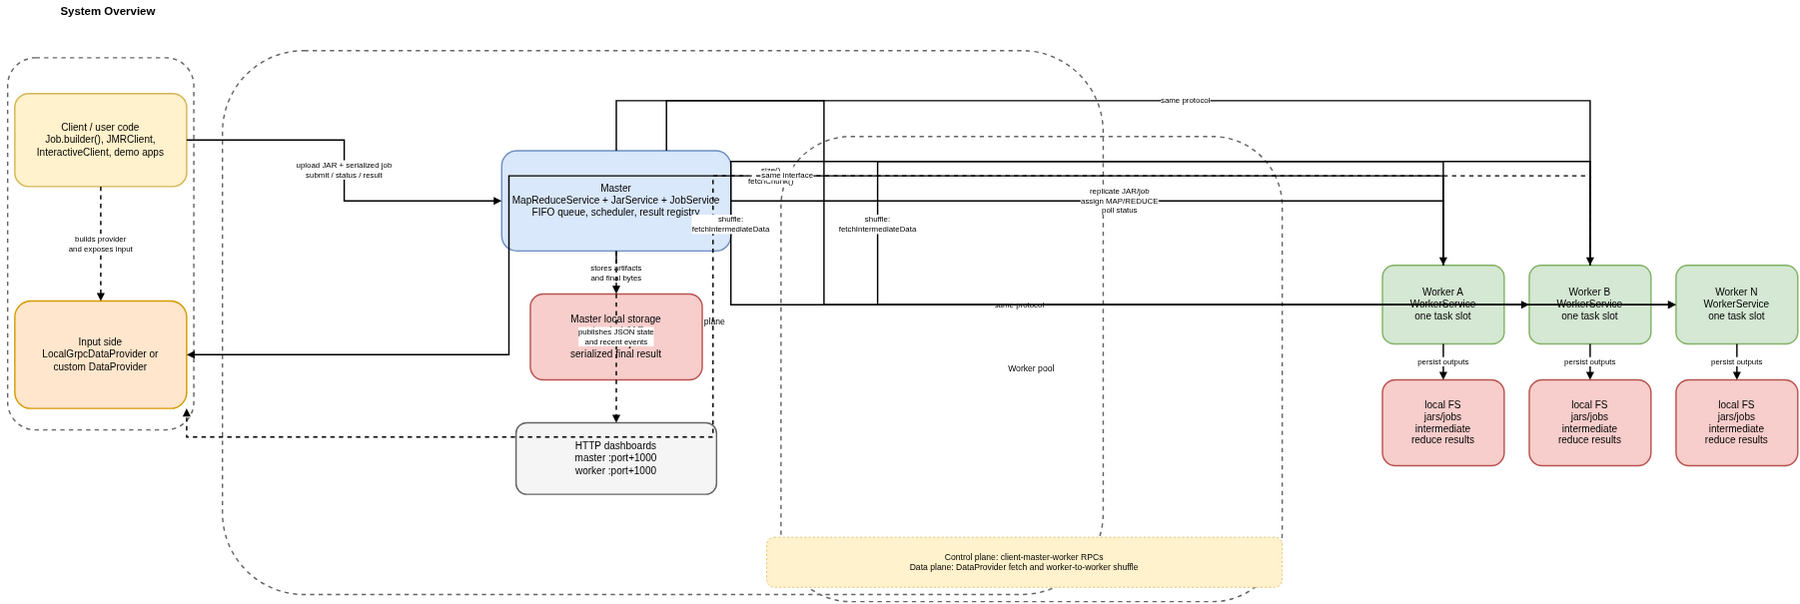
\includegraphics[width=0.95\textwidth]{diagrams/system_overview.png}
    \caption{High-level architecture of the implemented system}
    \label{fig:system-overview}
\end{figure}

\paragraph{Architectural style.}
The style is a combination of:
%
\begin{itemize}
    \item a \textbf{centralized coordinator} for scheduling, progress tracking, retries, and job lifecycle management;
    \item a \textbf{pool of homogeneous workers} that execute the same runtime and expose a uniform gRPC interface;
    \item a \textbf{service-oriented data source abstraction} through \texttt{DataProvider}/\texttt{DataProviderClient};
    \item a \textbf{peer-to-peer shuffle path} among workers for intermediate partitions.
\end{itemize}

\paragraph{Why this style.}
This combination directly supports the requirements identified in \cref{requirements}. A single master simplifies FIFO job execution, global progress computation, and failure handling. Worker-local storage avoids turning the master into a bandwidth bottleneck for shuffle traffic. The serializable data-provider handle allows the library to remain independent from any specific filesystem or database technology. Finally, restricting each worker to one task at a time makes the behaviour easy to reason about and matches the non-functional requirement that forbids oversubscription on workers.

\subsection{Infrastructure}\label{infrastructure}
The runtime introduces five infrastructural families:
%
\begin{itemize}
    \item one \textbf{client process}, typically the submitter application or the interactive CLI;
    \item one \textbf{data-provider process}, can be started by the client or it can be a wrapper over an existing service (e.g., a full fledged NFS);
    \item one \textbf{master server}, running the scheduling and artifact-ingestion services;
    \item \textbf{N worker servers}, all running the same code and exposing task-execution plus shuffle endpoints;
    \item one \textbf{HTTP dashboard} per master and per worker, used only for observability.
\end{itemize}

The deployment topology presented as a reference use case in the is shown in \cref{fig:deployment-topology}. In this Docker-based setup, the master and workers are individual containers attached to the same virtual network, while the submitter and the local data provider run on the host.

\begin{figure}[htbp]
    \centering
    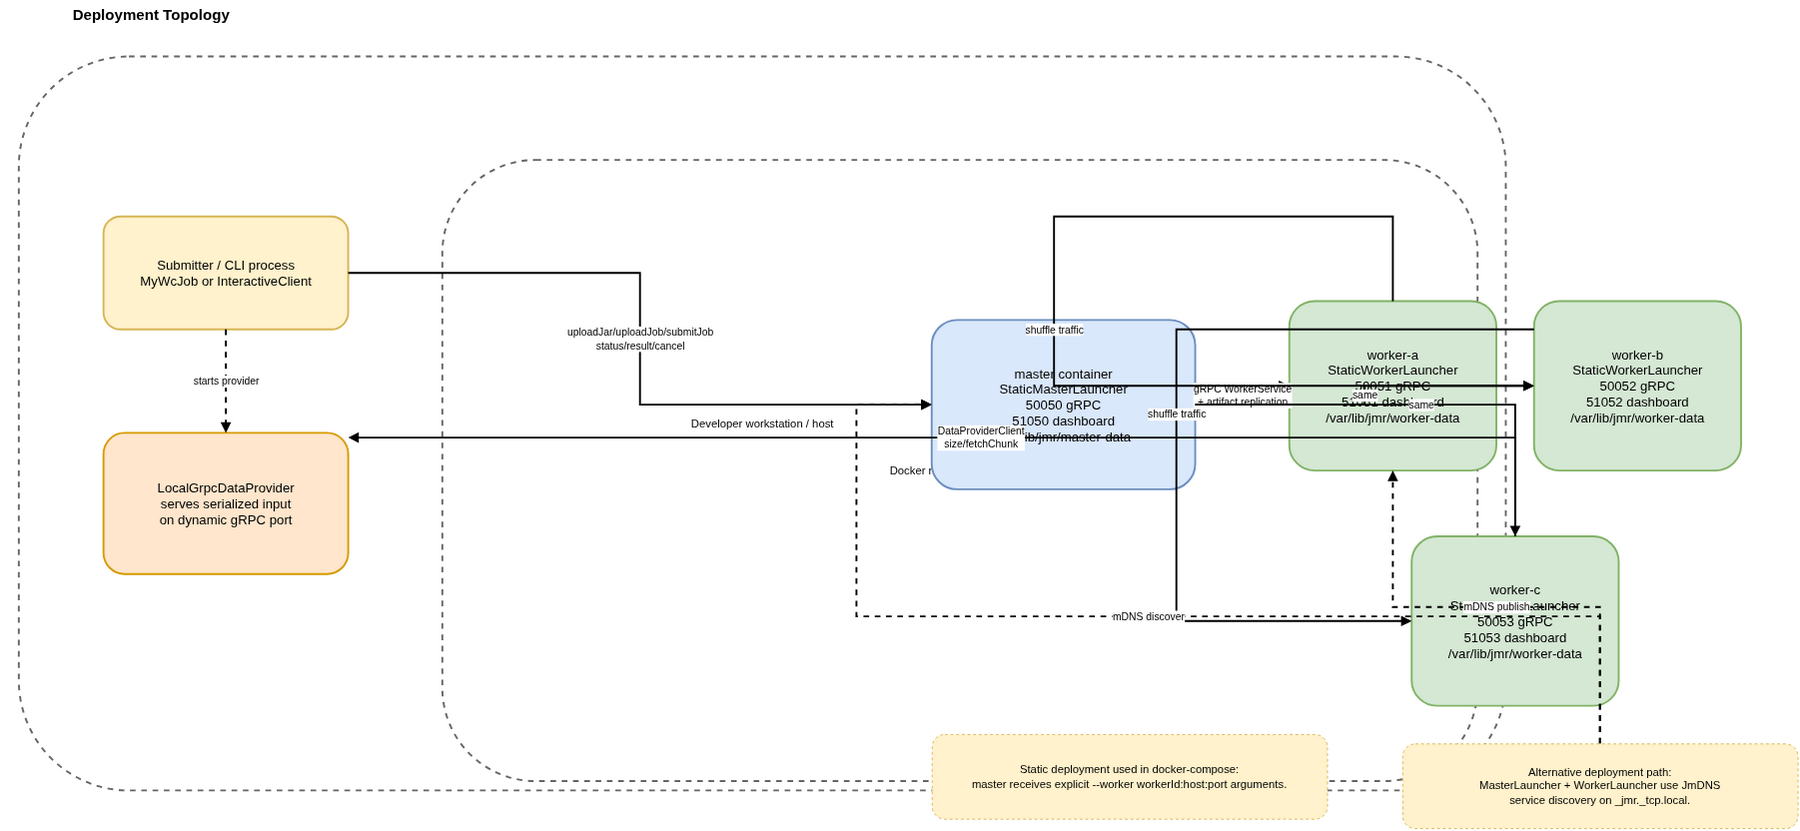
\includegraphics[width=0.95\textwidth]{diagrams/deployment_topology.png}
    \caption{Deployment topology used by the project scripts}
    \label{fig:deployment-topology}
\end{figure}

\paragraph{Distribution over the network.}
The master must be reachable by the client and by all workers. Workers must be mutually reachable as well, because the reduce phase fetches intermediate data directly from the worker that produced each partition. The data provider only needs to be reachable by the workers. This creates two practical communication channels:
%
\begin{itemize}
    \item \textbf{control traffic}: client-master and master-worker RPCs;
    \item \textbf{data traffic}: worker-data-provider and worker-worker shuffle RPCs.
\end{itemize}

\paragraph{How components find each other.}
Two mechanisms are implemented:
%
\begin{itemize}
    \item \textbf{static addressing}, used by \texttt{StaticMasterLauncher} and the Docker scripts, where the master receives explicit \texttt{workerId:host:port} triples;
    \item \textbf{JmDNS-based discovery}, used by \texttt{MasterLauncher} and \texttt{WorkerLauncher}, where workers publish themselves under \texttt{\_jmr.\_tcp.local.} and the master discovers them at startup.
\end{itemize}

Static addressing is the most deterministic option and is therefore used in local end-to-end runs. Service discovery is still useful to satisfy the requirement that the cluster can self-configure in non-containerized environments.

\subsection{Modelling}\label{modelling}
The core domain and runtime objects are summarized in \cref{fig:domain-model}. The most important modelling choice is that user code is not interpreted remotely through reflection-only metadata: instead, the system serializes a complete \texttt{JobConfiguration} object, distributes the corresponding fat JAR to all workers, deserializes the job and loads it dynamically in the classloader of the worker, locally, where it will execute.

\begin{figure}[htbp]
    \centering
    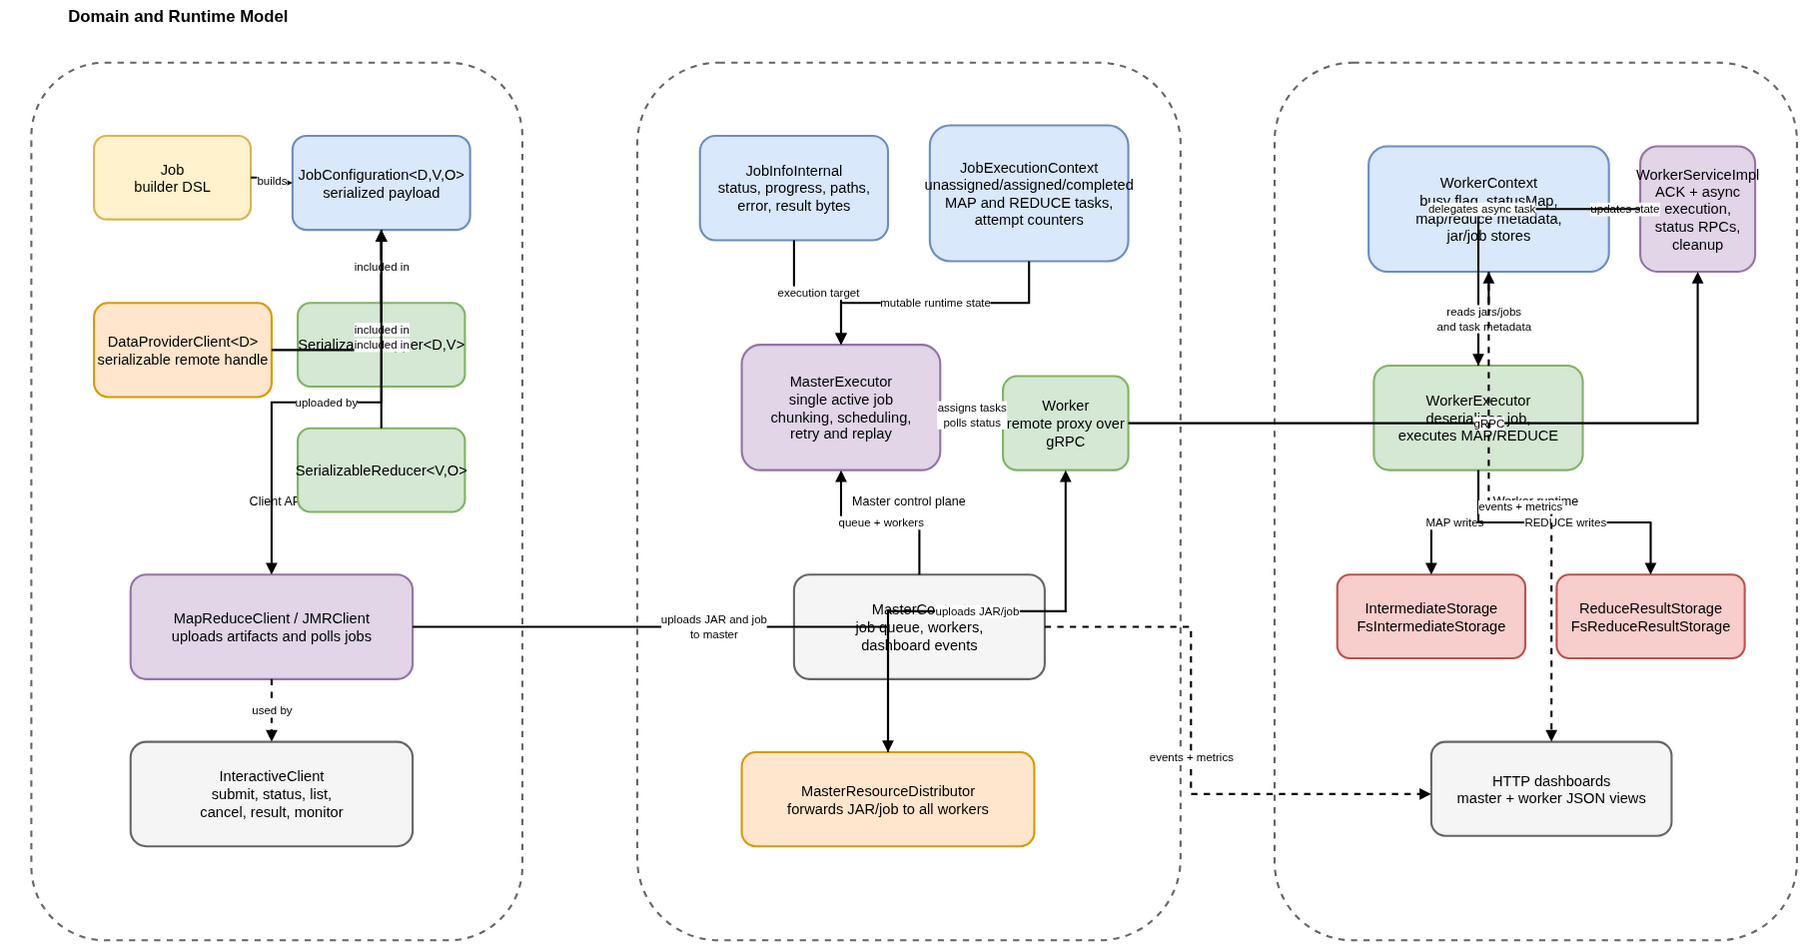
\includegraphics[width=0.95\textwidth]{diagrams/domain_model.png}
    \caption{Domain entities and their mapping to runtime components}
    \label{fig:domain-model}
\end{figure}

\paragraph{Main domain entities.}
%
\begin{description}
    \item[\texttt{JobConfiguration<D,V,O>}] the serializable descriptor of one MapReduce job. It contains a \texttt{DataProviderClient}, a mapper, and a reducer.
    \item[\texttt{JobInfoInternal}] the master-side representation of a submitted job: status, progress, storage paths, error message, execution timestamps, and serialized final result.
    \item[\texttt{Unassigned/Assigned/Completed MapTasks}] the three views used by the master to manage map scheduling and completion.
    \item[\texttt{Unassigned/Assigned/Completed ReduceTasks}] the analogous structures for the reduce phase.
    \item[\texttt{IntermediateLocation}] a logical pointer to one intermediate partition stored on a specific worker.
    \item[\texttt{Worker}] the master-side remote proxy wrapping the gRPC stubs of one worker.
    \item[\texttt{WorkerContext}] the local runtime state of a worker: busy flag, task-status map, storage directories, recent results, and dashboard events.
\end{description}

\subsection{Interaction}\label{interaction}
The dominant interaction pattern is a mix of \textbf{command, asynchronous completion, polling}. A task-submission RPC only means ``the worker accepted the task''; it does \emph{not} mean ``the task has completed''. Completion is observed later through periodic status polling by the master. This pattern keeps RPC handlers short, prevents long-lived blocking calls, and matches the one-task-per-worker design.

\paragraph{Job submission and bootstrap.}
\cref{fig:job-submission-sequence} shows the startup path of a job. The client first uploads the JAR, then uploads the serialized \texttt{JobConfiguration}, and only afterwards calls \texttt{submitJob(jarId, jobId)}. As soon as the master receives the JAR and job bytes, it forwards them to all currently known workers through \texttt{MasterResourceDistributor}. Therefore, by the time execution starts, every worker already has both the code and the serialized configuration locally available.

\begin{figure}[htbp]
    \centering
    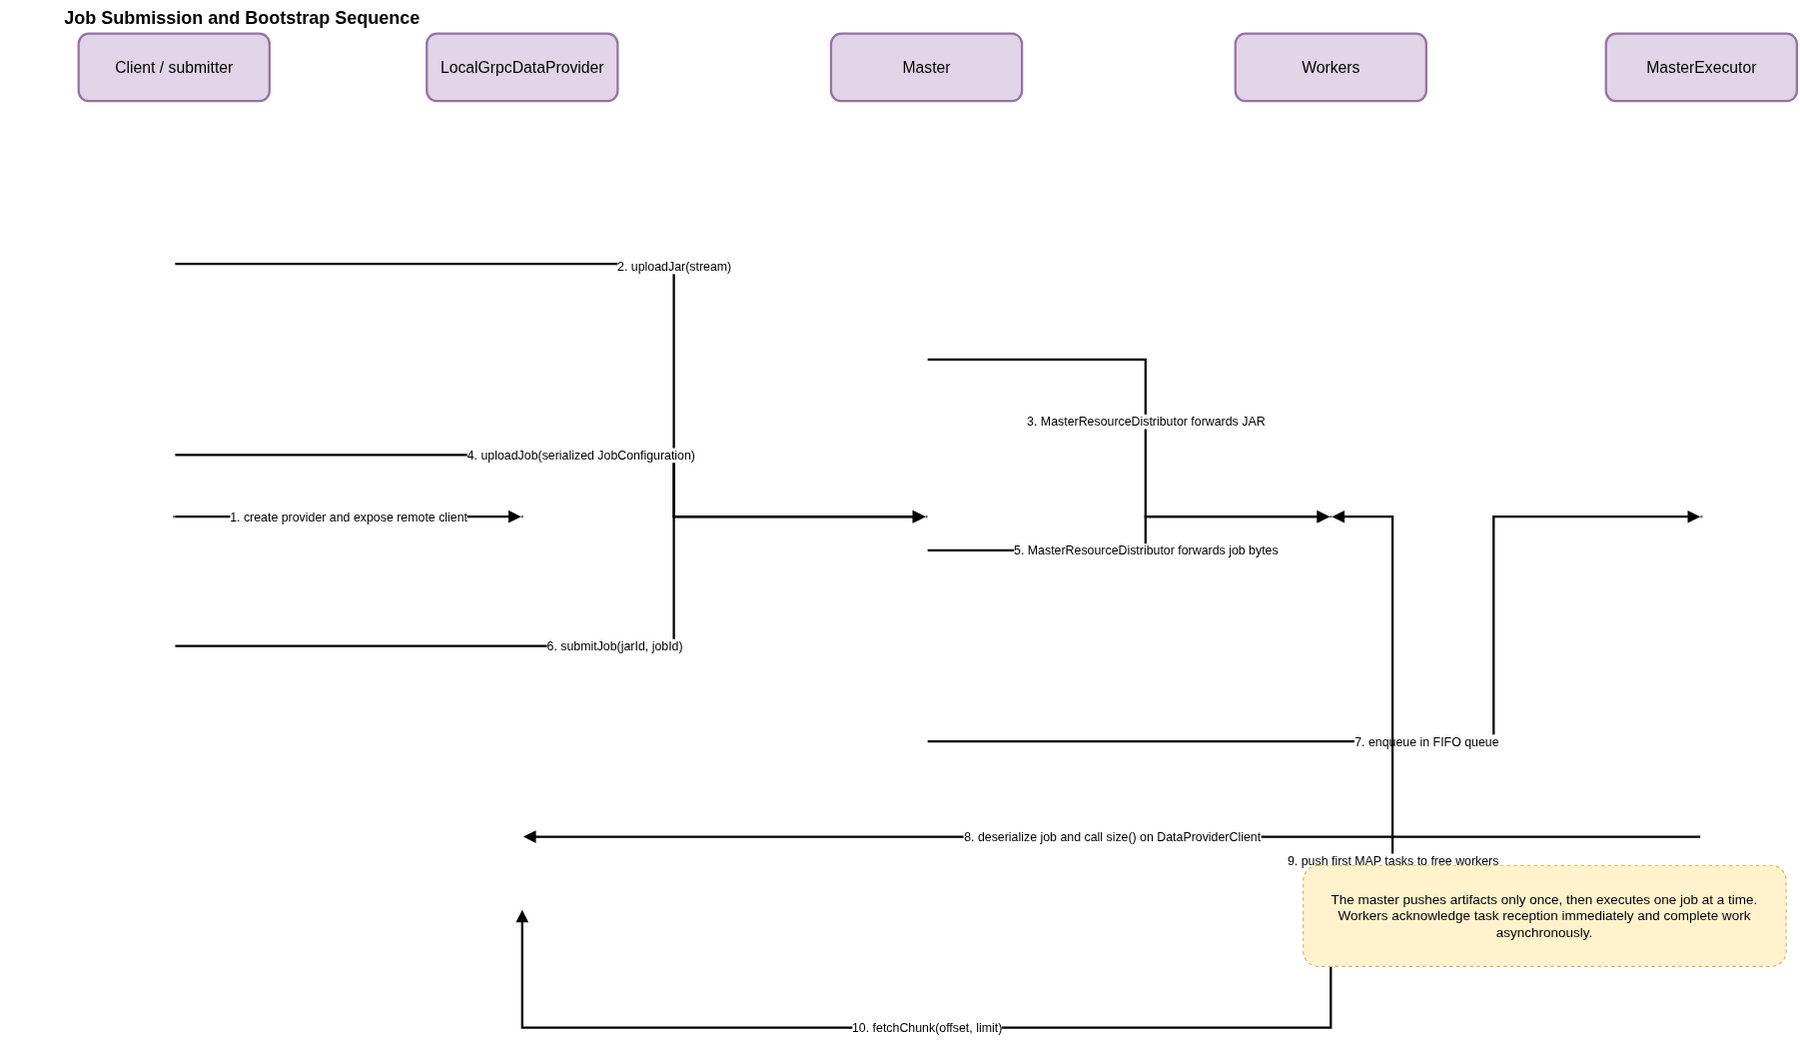
\includegraphics[width=0.95\textwidth]{diagrams/job_submission_sequence.png}
    \caption{Sequence of job submission, artifact distribution, and first task assignment}
    \label{fig:job-submission-sequence}
\end{figure}

\paragraph{User-facing interaction points.}
At the system boundary, the implementation exposes more than one interface, as shown in \cref{fig:user-surfaces}. The primary interface is the programmatic API used by client applications. On top of that, the repository also provides a CLI shell and lightweight dashboards. This is useful because the project is a library, but during validation and deployment an operator still needs direct observability and manual control.

\begin{figure}[htbp]
    \centering
    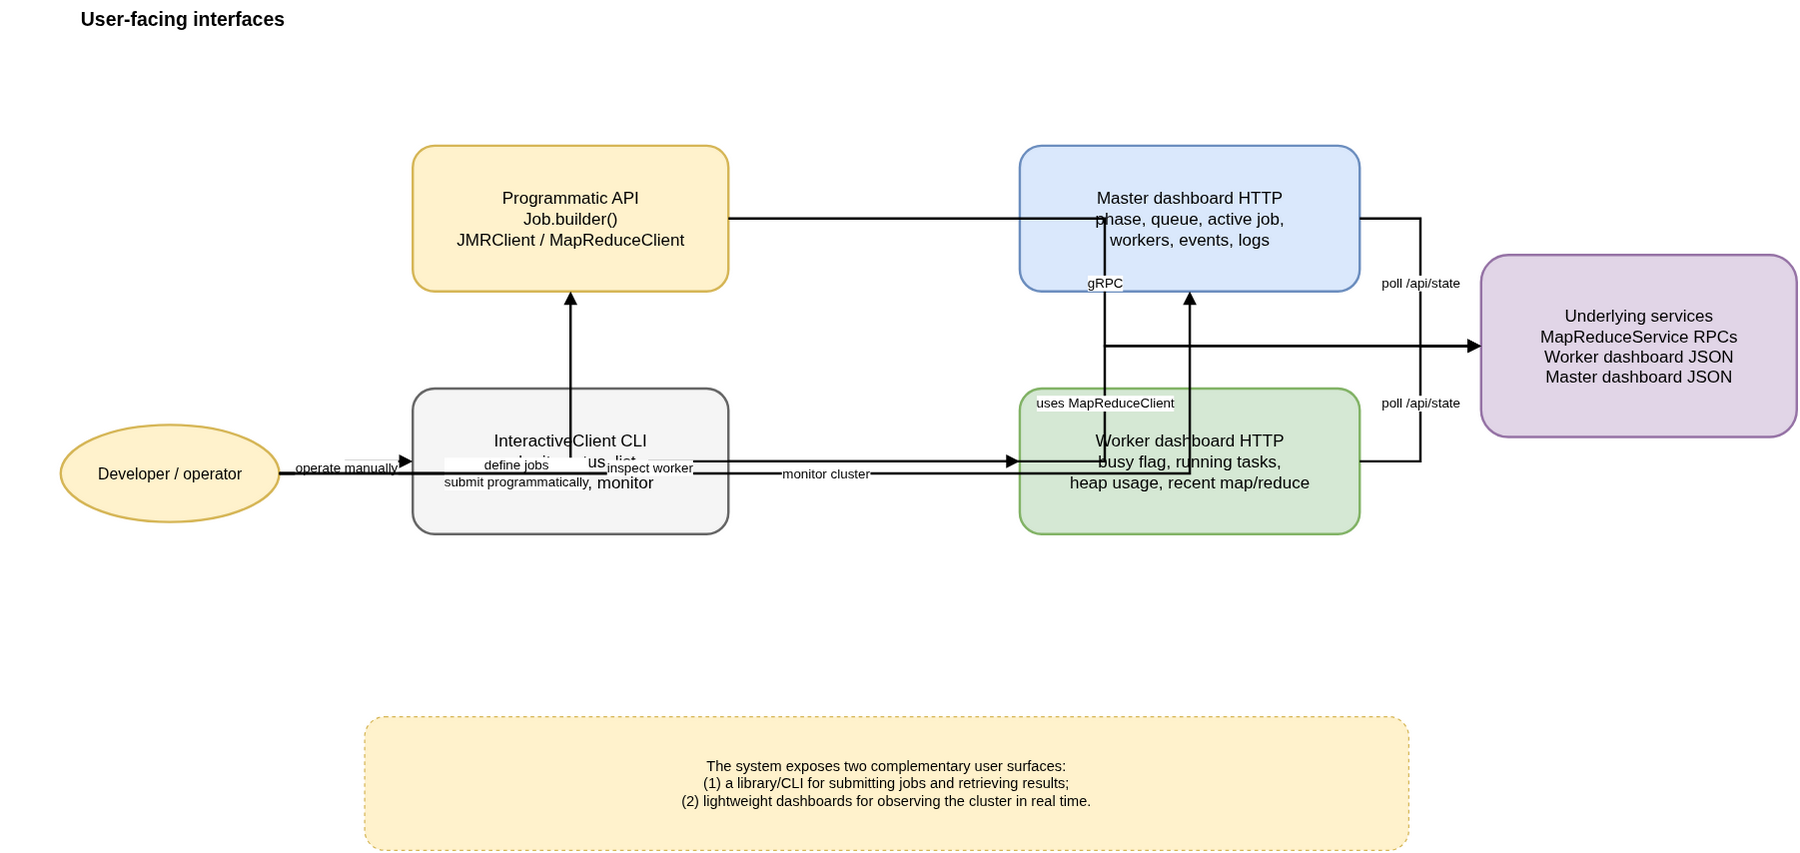
\includegraphics[width=0.95\textwidth]{diagrams/user_surfaces.png}
    \caption{User-facing interfaces exposed by the project}
    \label{fig:user-surfaces}
\end{figure}

\paragraph{Protocol choices in the interaction layer.}
All control and data RPCs among distributed components use gRPC with Protocol Buffers. The only exception is observability: dashboards use a tiny HTTP server that exposes a JSON snapshot consumed by an auto-refreshing HTML page. This keeps the operational interface simple and decoupled from the execution path.

\subsection{Behaviour}\label{behaviour}
The end-to-end algorithm executed by the system is summarized in \cref{fig:map-reduce-flow}. The figure is intentionally more detailed than the architectural views: it describes the concrete scheduling and data-processing steps implemented in the code, not an abstract MapReduce textbook pipeline.

\begin{figure}[htbp]
    \centering
    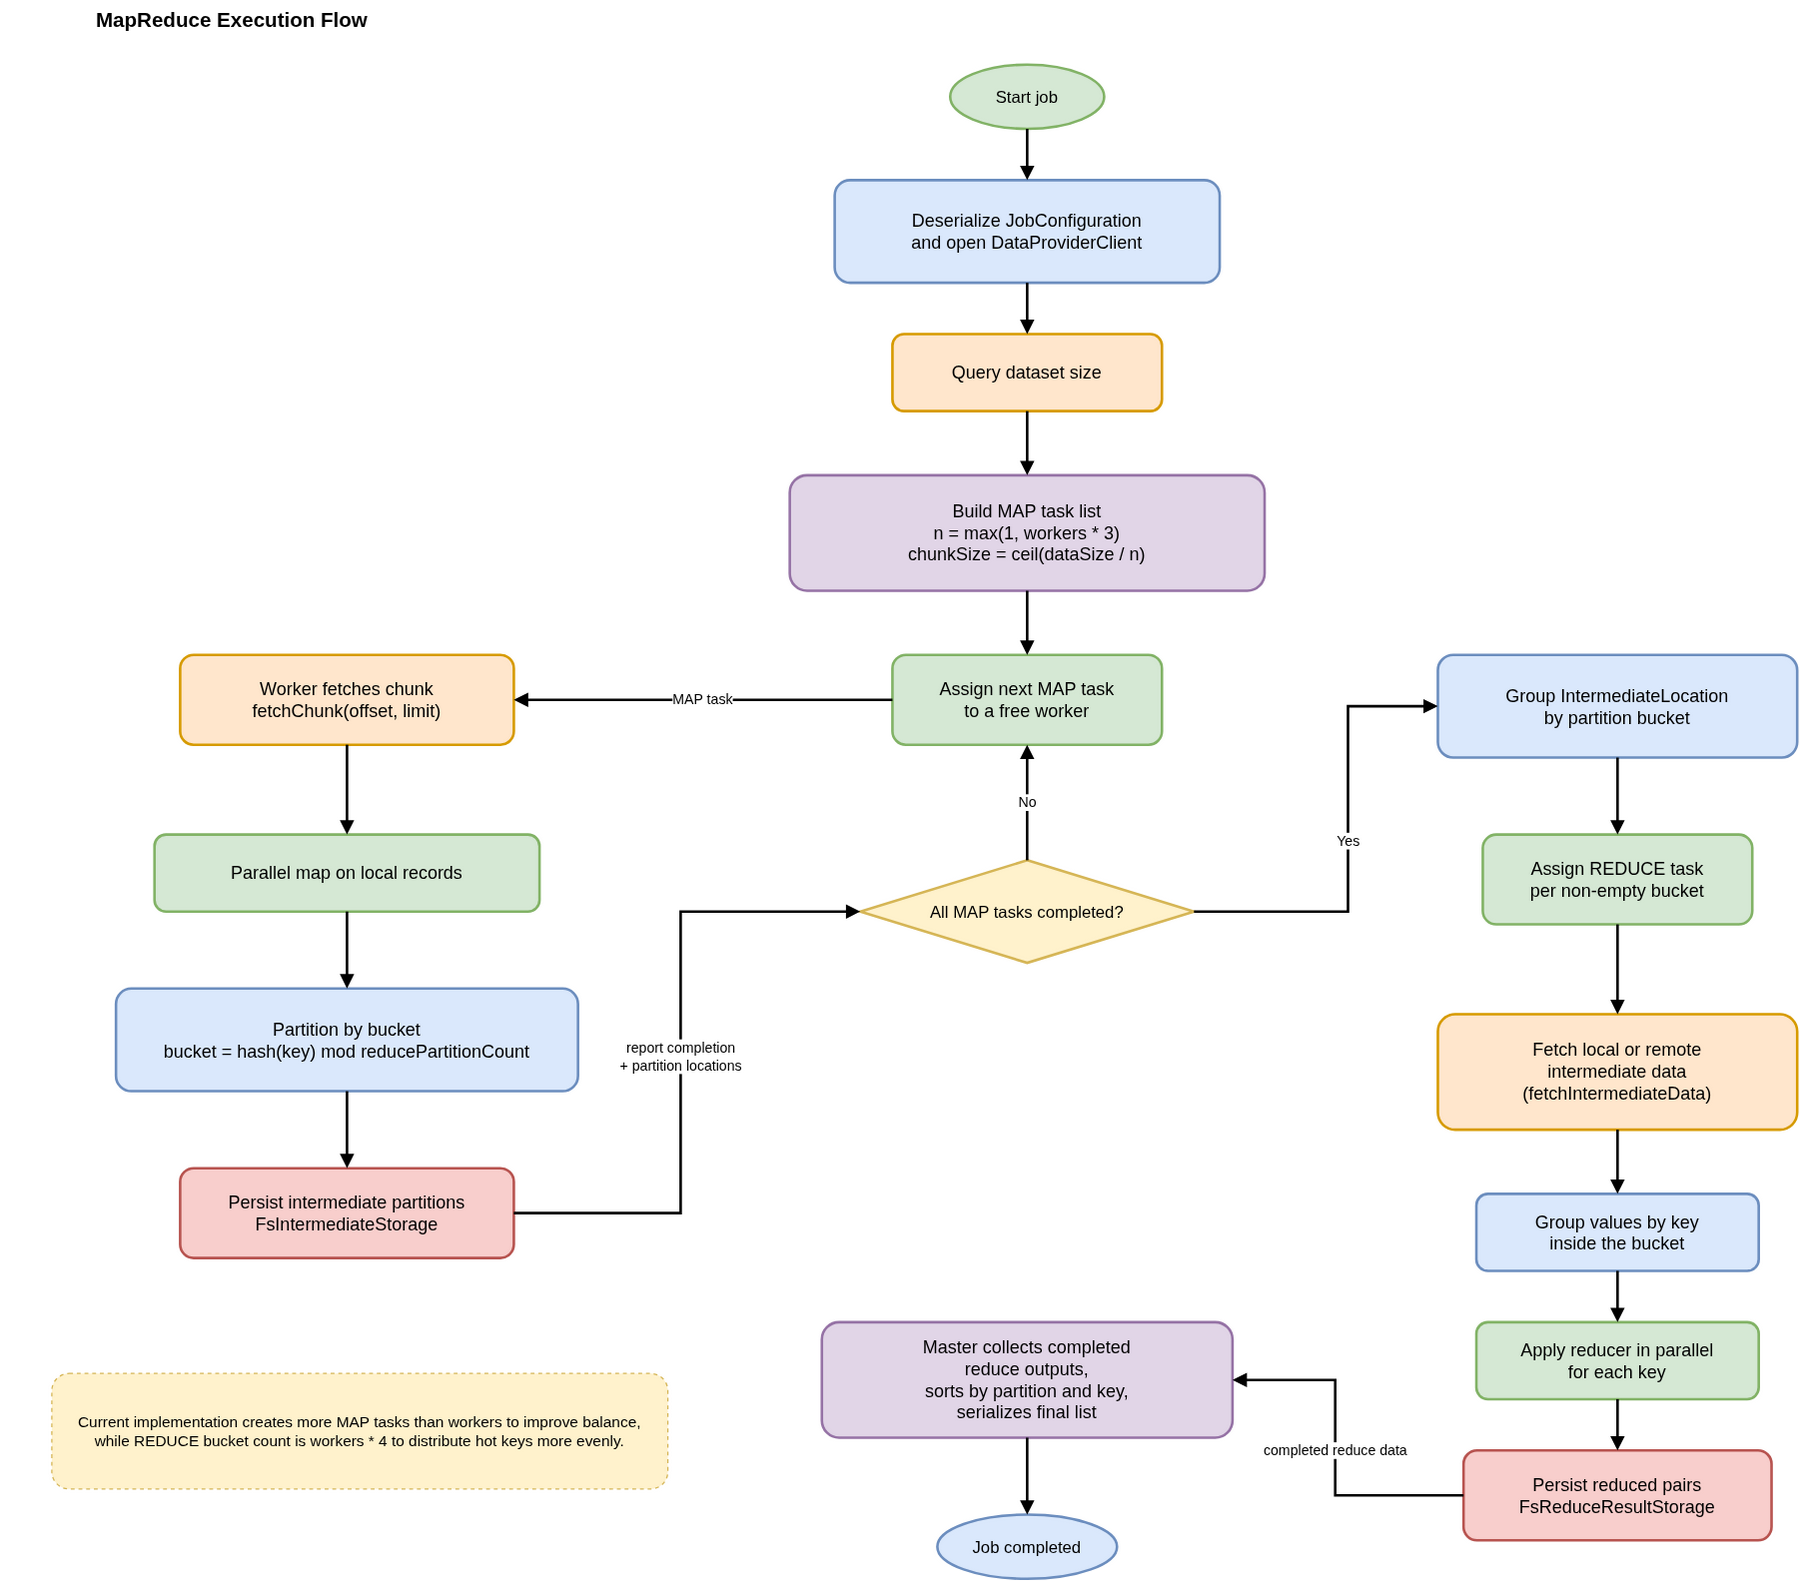
\includegraphics[width=0.92\textwidth]{diagrams/map_reduce_flow.png}
    \caption{Detailed behaviour of the implemented MapReduce execution pipeline}
    \label{fig:map-reduce-flow}
\end{figure}

The observable lifecycle of a job is shown in \cref{fig:job-lifecycle-state}. This state-oriented view complements the data-flow diagram by making explicit the difference between the public job status exposed to clients and the internal execution phases tracked by the master dashboard.

\begin{figure}[htbp]
    \centering
    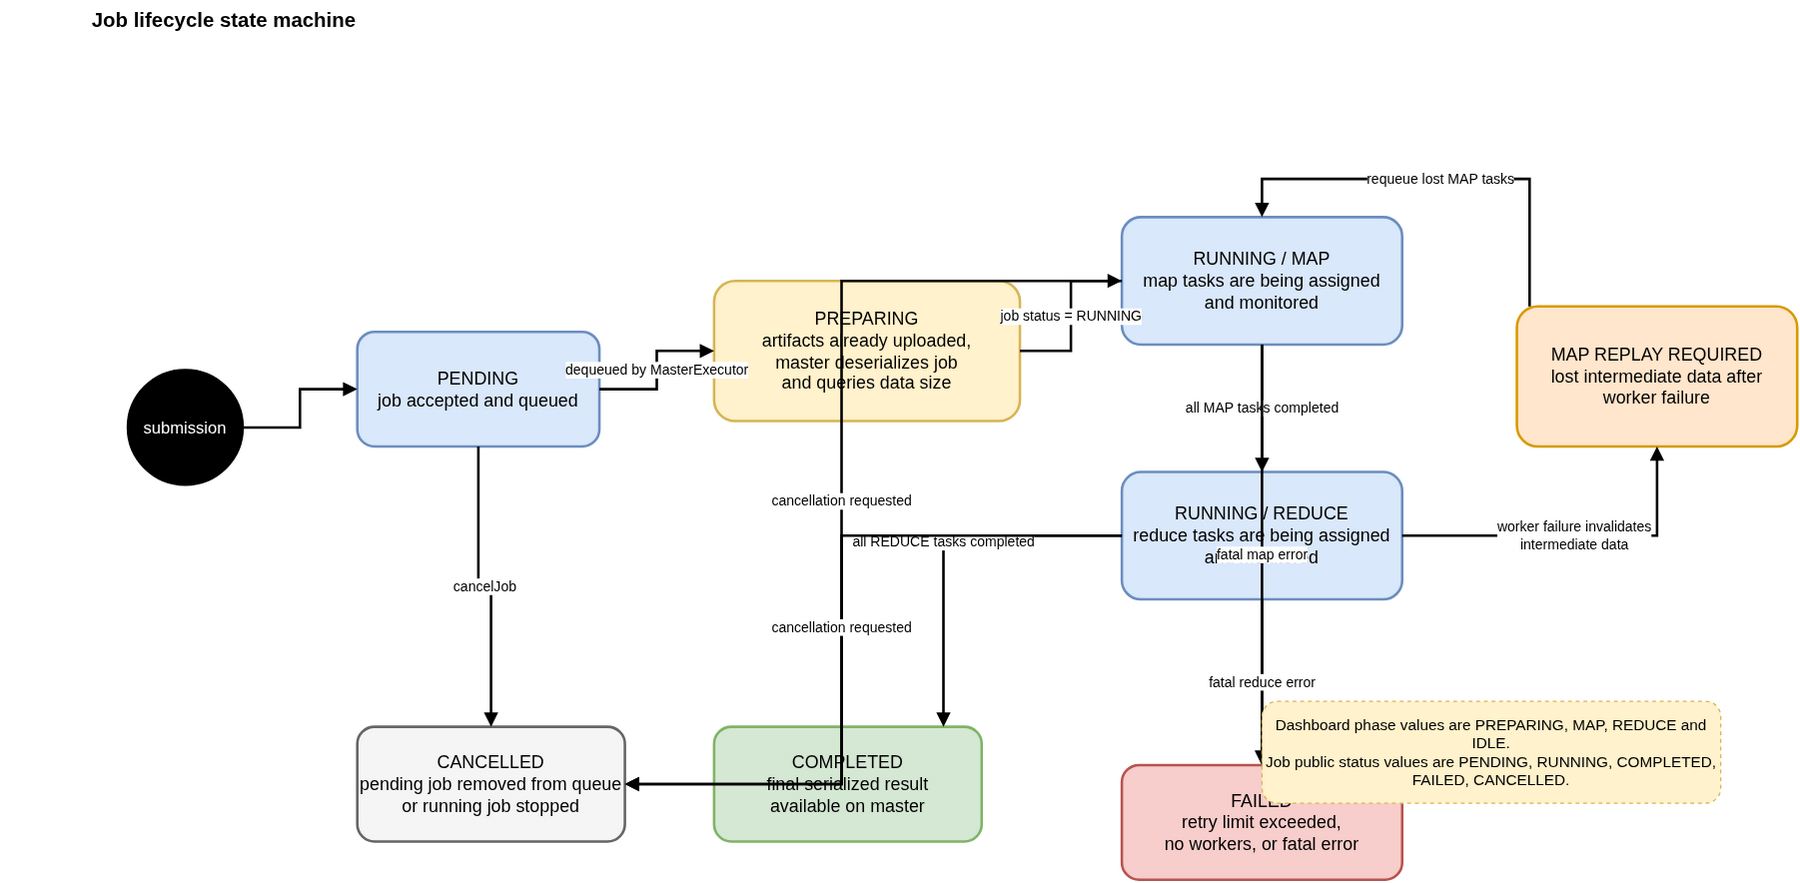
\includegraphics[width=0.9\textwidth]{diagrams/job_lifecycle_state.png}
    \caption{State machine of job execution}
    \label{fig:job-lifecycle-state}
\end{figure}

\paragraph{Master-side scheduling algorithm.}
The master updates the global state of the system. More precisely:
%
\begin{enumerate}
    \item it dequeues one job at a time from the FIFO queue;
    \item it deserializes the uploaded \texttt{JobConfiguration} using the uploaded JAR;
    \item it opens the \texttt{DataProviderClient} and queries the input size;
    \item it creates the map-task list by oversplitting the input into \(\max(1, 3 \cdot W)\) chunks, where \(W\) is the number of currently available workers, so that balancing is finer than the worker count;
    \item it continuously assigns unassigned tasks to the first healthy worker that is not already busy in the current phase;
    \item it polls task status until the phase completes, then computes the next phase;
    \item it serializes the final reduce outputs and stores the resulting byte array in the job metadata.
\end{enumerate}

The choice of producing more map tasks than workers is deliberate: it mitigates skew when input chunks have different processing cost. Reduce partitioning is also finer-grained than the worker count. The current implementation uses
\[
    \texttt{reducePartitionCount} = \max(1, W \cdot \texttt{REDUCE\_BUCKETS\_PER\_WORKER})
\]
with \texttt{REDUCE\_BUCKETS\_PER\_WORKER = 4}. This makes hot keys less likely to concentrate all work on a single worker.

\paragraph{Worker-side map algorithm.}
When a worker receives a map task, it first tries to acquire a local task slot through an atomic busy flag. If the worker is already executing something, it rejects the task immediately. Otherwise, it acknowledges the RPC and starts the real work asynchronously on a single-thread executor. The map algorithm executed by the worker is:
%
\begin{enumerate}
    \item deserialize the \texttt{JobConfiguration} from local JAR and job files;
    \item initialize the remote \texttt{DataProviderClient};
    \item fetch the input chunk identified by \texttt{offset} and \texttt{limit};
    \item apply the mapper in parallel over the local records;
    \item partition each emitted key-value pair into a reduce bucket using
          \[
              \texttt{bucket} = \texttt{floorMod(key.hashCode(), reducePartitionCount)};
          \]
    \item persist each bucket as a compressed serialized file in \texttt{FsIntermediateStorage};
    \item expose the resulting \texttt{IntermediateLocation} list to the master via \texttt{GetMapTaskStatus}.
\end{enumerate}

\paragraph{Shuffle and reduce algorithm.}
After the map phase, the master groups all \texttt{IntermediateLocation} objects by bucket id and creates one reduce task per non-empty bucket. A worker executing a reduce task then:
%
\begin{enumerate}
    \item fetches the intermediate fragments referenced by that bucket;
    \item reads them locally if the producing worker is itself, or remotely through streaming \texttt{fetchIntermediateData} if they live elsewhere;
    \item groups all received pairs by key using concurrent collectors;
    \item applies the reducer in parallel over each key group;
    \item persists the reduced list in \texttt{FsReduceResultStorage};
    \item serves the reduced pairs back to the master when \texttt{GetReduceTaskStatus} is polled.
\end{enumerate}

\paragraph{Behavioural invariants.}
Three invariants are particularly important:
%
\begin{itemize}
    \item the master executes at most one job at a time;
    \item each worker executes at most one task at a time;
    \item map and reduce outputs become immutable as soon as the corresponding task is marked completed.
\end{itemize}

These invariants greatly simplify reasoning about correctness, retries, and cleanup.

\subsection{Data and Consistency Issues}\label{data-and-consistency-issues}
The implementation does \emph{not} use a database. The stored data are temporary execution artifacts and final result bytes:
%
\begin{itemize}
    \item on the \textbf{master}: uploaded JAR files, uploaded serialized job files, in-memory job metadata, and the final serialized result;
    \item on each \textbf{worker}: a local copy of the JARs and job files needed for execution, compressed intermediate partitions, and compressed reduce results;
    \item outside the cluster, behind the \textbf{data provider}: the original input dataset.
\end{itemize}

\paragraph{Storage model.}
All persisted execution data are stored as local files, not as rows in a DBMS. This is coherent with the requirements: the library only needs transient per-job state, not multi-tenant transactional records. Using the local filesystem keeps the runtime simple and avoids introducing a database dependency only for ephemeral task outputs.

\paragraph{Shared data.}
There are three kinds of shared data:
%
\begin{itemize}
    \item \textbf{job artifacts} (JAR and serialized job), replicated from master to workers;
    \item \textbf{intermediate locations}, owned by the master as metadata but referring to files owned by workers;
    \item \textbf{final result bytes}, stored by the master and later downloaded by the client.
\end{itemize}

\paragraph{Consistency strategy.}
Consistency is mostly achieved by architecture rather than by a complex protocol:
%
\begin{itemize}
    \item the master is the single writer of global job state;
    \item task outputs are immutable after completion;
    \item workers never concurrently write the same task output path, because task ids are unique and workers run one task at a time;
    \item the final result is made deterministic by sorting completed reduce partitions and then sorting the emitted pairs by key before serialization.
\end{itemize}

This last point is important for reproducibility: even if execution order differs between runs, the final serialized list follows a stable ordering.

\subsection{Fault-Tolerance}\label{fault-tolerance}
Fault tolerance is intentionally asymmetric: \textbf{worker failures are tolerated}, \textbf{master failures are not}. This matches the requirements and keeps the implementation manageable. The concrete recovery logic is summarized in \cref{fig:fault-tolerance-sequence}.

\begin{figure}[htbp]
    \centering
    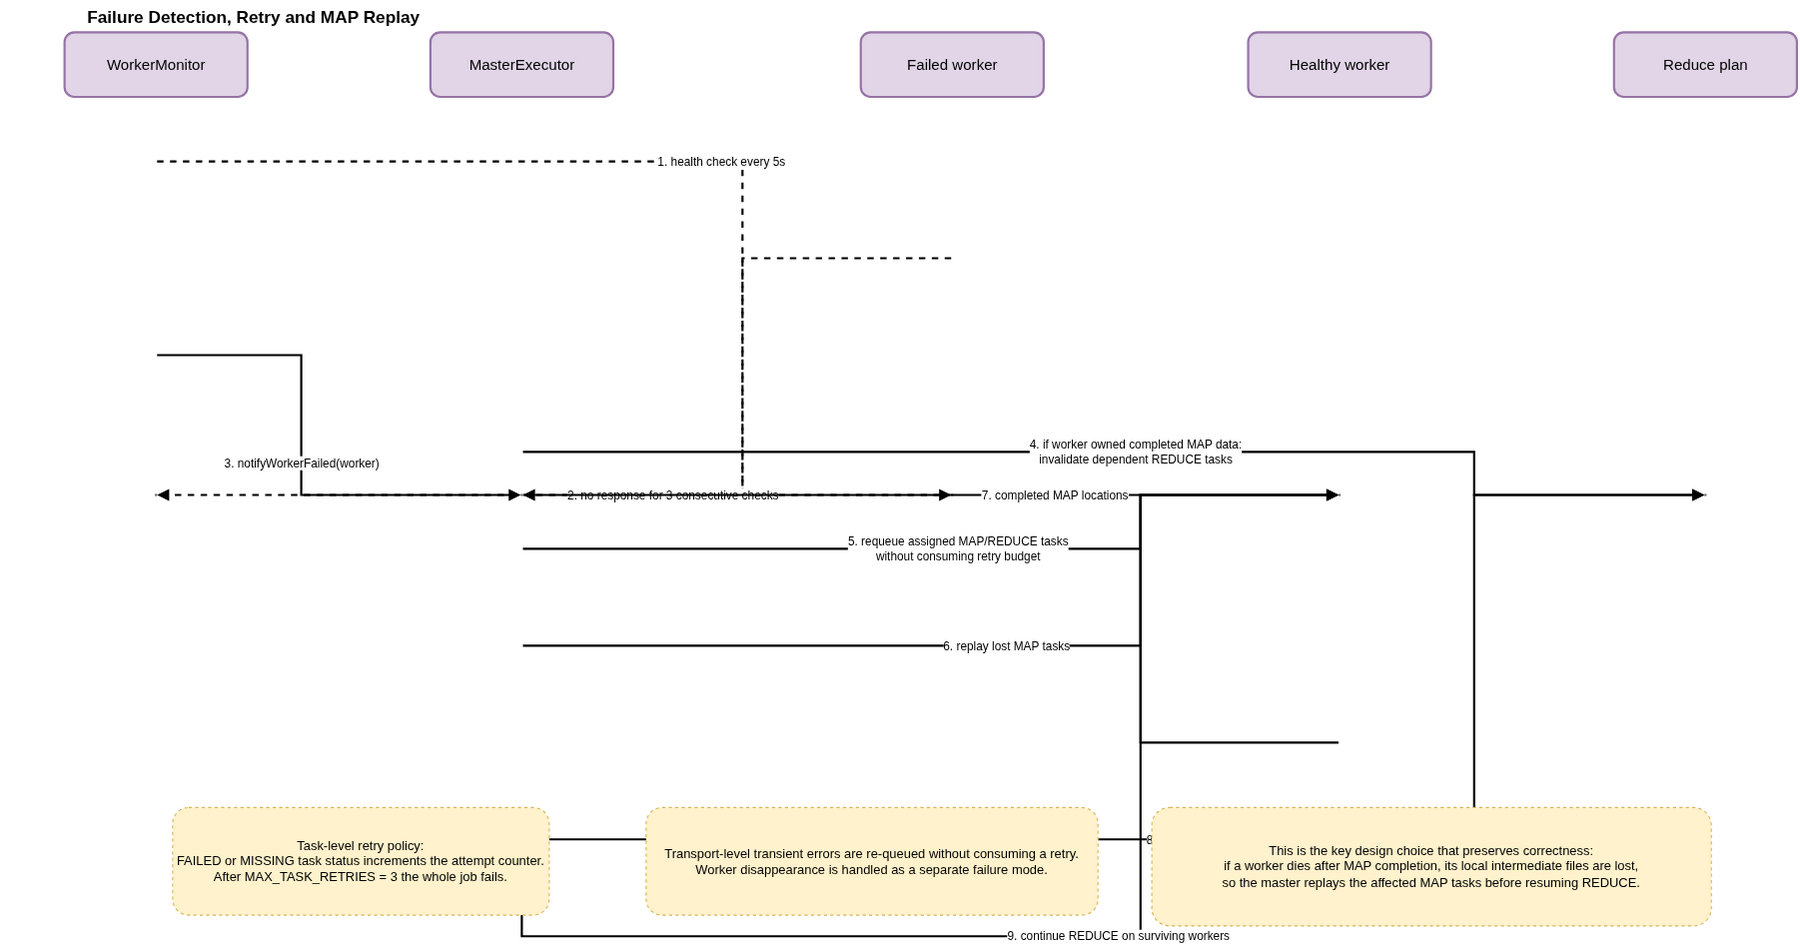
\includegraphics[width=0.95\textwidth]{diagrams/fault_tolerance_sequence.png}
    \caption{Failure detection, retry, and map replay after loss of intermediate data}
    \label{fig:fault-tolerance-sequence}
\end{figure}

\paragraph{Artifact replication.}
The master replicates uploaded JARs and serialized job files to all workers as soon as they are received. This is not data replication in the distributed-filesystem sense, but it is still a form of replication that serves two purposes:
%
\begin{itemize}
    \item workers can start executing immediately when assigned a task;
    \item job execution does not depend on the client keeping the original JAR or serialized object available.
\end{itemize}

\paragraph{Liveness detection.}
The implementation contains a \texttt{Heartbeat} RPC in the protocol, but the deployed failure detector is actually \textbf{master-driven active health checking}. \texttt{WorkerMonitor} probes the gRPC health service every 5 seconds and removes a worker only after \texttt{WORKER\_HEALTH\_FAILURE\_THRESHOLD = 3} consecutive failures. In practice, a worker is therefore considered dead after about 15 seconds of unreachability. This design is simpler than a push-based heartbeat loop and reuses the standard gRPC health mechanism.

\paragraph{Retry policy.}
Task re-execution follows a precise policy:
%
\begin{itemize}
    \item if a worker is \textbf{busy}, it rejects the task immediately; the task stays queued and no retry is consumed;
    \item if the master polls a task and receives \texttt{FAILED} or \texttt{MISSING}, the task is re-queued and its retry counter is incremented;
    \item if a non-fatal gRPC error occurs while polling, the task is re-queued without consuming a retry;
    \item if retries exceed \texttt{MAX\_TASK\_RETRIES = 3}, the whole job fails.
\end{itemize}

\paragraph{Worker crash during map or reduce.}
If a worker disappears while it owns \emph{assigned} tasks, those tasks are simply moved back to the unassigned queue and can be executed by a surviving worker. This case is conceptually straightforward.

\paragraph{Worker crash after map completion.}
The subtle case is losing a worker \emph{after} it completed one or more map tasks. In this system, intermediate partitions are stored only on the worker that produced them. Therefore, if such a worker dies during the reduce phase, some reduce inputs become unavailable. The master reacts as follows:
%
\begin{enumerate}
    \item remove the completed map tasks whose intermediate files were lost;
    \item re-queue those map tasks for re-execution on surviving workers;
    \item invalidate any reduce tasks that depend on the lost partitions;
    \item wait for the replayed map tasks to complete;
    \item rebuild the reduce-task list from the new intermediate locations;
    \item restart the reduce phase.
\end{enumerate}

This is the key recovery mechanism of the project. It replaces storage replication with deterministic re-execution, which is a reasonable tradeoff for an educational MapReduce library.

\paragraph{Cleanup and error handling.}
After termination, the master asks every reachable worker to remove local artifacts for the completed job. If cleanup on a specific worker fails because the worker is already unreachable, the failure is logged but does not alter the job outcome. If all workers disappear, or if retries are exhausted, the job is marked as failed and the error message is stored in \texttt{JobInfoInternal}.

\subsection{Availability}\label{availability}
There is no traditional cache such as Redis or a replicated in-memory key-value store. However, the implementation still benefits from two small reuse mechanisms:
%
\begin{itemize}
    \item workers and worker servers reuse gRPC channels and blocking stubs when fetching remote intermediate data;
    \item intermediate and reduced outputs remain locally available until the final cleanup step, so repeated status polling does not require recomputation.
\end{itemize}

\paragraph{Load balancing.}
Load balancing is achieved by scheduling strategy rather than by a dedicated balancer component:
%
\begin{itemize}
    \item the map phase creates more tasks than workers (\(3 \cdot W\)), which reduces skew;
    \item the master assigns a task to the first healthy worker that is not already busy;
    \item each worker enforces local admission control by accepting at most one task at a time.
\end{itemize}

This policy is simple, but effective for the intended setting. It does not need resource estimation, speculative execution, or work stealing to keep the cluster reasonably utilized.

\paragraph{Network partitioning.}
From the master's point of view, a network partition affecting one or more workers is indistinguishable from worker unavailability. After the failure threshold is exceeded, those workers are removed from the available set and their tasks are re-queued or replayed. If at least one worker remains reachable, the job can still complete. If the partition isolates the master from all workers, the active job eventually fails because no healthy worker remains. There is no split-brain scenario, since there is only one master and workers never elect a replacement.

\subsection{Security}\label{security}
Security is intentionally minimal in the current implementation.

\paragraph{Authentication and authorization.}
There is no built-in authentication among client, master, workers, or data provider. Likewise, there is no authorization model with roles or access rights. Any process that can reach the exposed ports and speak the expected protocol can upload artifacts or query status. This is acceptable only under the project assumption of a trusted deployment environment.

\paragraph{Cryptography.}
gRPC channels are created in plaintext mode, and the dashboards are plain HTTP endpoints. No TLS, token verification, or signed-artifact validation is enforced by the library itself. The uploaded JAR contains arbitrary executable code that will run on all workers, so the trust boundary is essentially the whole cluster.

\paragraph{Practical implication.}
The system should therefore be deployed only on controlled networks, such as a development machine, a protected Docker bridge, or a private datacenter/VPC segment. In a production-grade evolution of this project, the minimum security additions would be mutual TLS on gRPC channels, authenticated job submission, and artifact validation before execution.

\section{Implementation}\label{implementation}
This section documents the technology-dependent choices made during implementation. In a few places the final implementation intentionally diverges from the original requirement discussion. The most important example is storage: the requirements initially emphasized in-memory processing, while the implemented runtime persists intermediate and reduced outputs on local worker disks to simplify recovery, cleanup, and observability.

\paragraph{Network protocols.}
The project uses \textbf{gRPC over HTTP/2} for all distributed control and execution traffic:
%
\begin{itemize}
    \item client-master RPCs for artifact upload, job submission, status retrieval, cancellation, and result download;
    \item master-worker RPCs for task assignment, task-status polling, and cleanup;
    \item worker-worker RPCs for shuffle data transfer;
    \item worker-data-provider RPCs for input-size queries and chunk retrieval.
\end{itemize}

Service discovery, when enabled, is implemented through \textbf{JmDNS}/mDNS rather than through a dedicated registry. Observability is intentionally separated from the execution path and uses a minimal \textbf{HTTP} server that publishes JSON snapshots consumed by a static HTML page.

\paragraph{Representation of in-transit data.}
Different data classes use different representations according to their role:
%
\begin{itemize}
    \item \textbf{Protocol Buffers} encode the gRPC request/response messages;
    \item \textbf{Java native serialization} is used for user-defined job configuration, mapped values, reduced values, and \texttt{DataProviderClient} objects;
    \item \textbf{GZIP-compressed serialized payloads} are used for persisted intermediate partitions and reduce outputs, and also for streamed shuffle batches;
    \item \textbf{JSON} is used only by the master and worker dashboards.
\end{itemize}

This mixed approach is pragmatic. Protocol Buffers keep service contracts explicit and compact, while Java serialization is the simplest way to move arbitrary user code and user-defined data types across the cluster.

\paragraph{Persistence model.}
No relational or NoSQL database is queried by the runtime. The implemented system relies on:
%
\begin{itemize}
    \item concurrent in-memory maps for job metadata and runtime bookkeeping;
    \item the local filesystem of the master for uploaded artifacts and final result bytes;
    \item the local filesystem of each worker for replicated artifacts, intermediate partitions, and reduced task outputs.
\end{itemize}

This choice reduces operational complexity and is sufficient because the system is single-tenant, executes one job at a time, and only needs ephemeral execution state rather than long-term transactional data.

\paragraph{Authentication and authorization in practice.}
The implementation currently performs neither authentication nor authorization. Component identity is therefore based only on network reachability and, in the static deployment mode, on explicit host/port configuration. This was acceptable for the project scope, but it is clearly a limitation and is discussed further in \cref{future-works}.

\subsection{Technological details}\label{technological-details}
The main technologies and libraries exploited by the implementation are the following:
%
\begin{itemize}
    \item \textbf{Java 21} as source and target language level for the Maven modules;
    \item \textbf{Maven} for multi-module build orchestration, assembly of fat JARs, and test execution;
    \item \textbf{gRPC 1.46.0} and \textbf{Protocol Buffers 3.24.0} for all remote service APIs;
    \item \textbf{JmDNS} for optional zero-configuration worker discovery;
    \item \textbf{SLF4J + Log4j2} for logging, with log streams also mirrored into the dashboards;
    \item \textbf{\texttt{com.sun.net.httpserver.HttpServer}} for the lightweight master and worker web dashboards;
    \item \textbf{Docker} for containerized runtime images, reproducible cluster deployment, and production-like integration testing;
    \item \textbf{JUnit 5} for Java unit tests and \textbf{Python 3} for top-level orchestration and integration tests.
\end{itemize}

From an engineering perspective, three implementation details are worth highlighting:
%
\begin{itemize}
    \item the cluster runtime is distributed as fat JARs so that user-defined mappers, reducers, and their dependencies can be deserialized safely on remote workers;
    \item worker execution is asynchronous with respect to the incoming RPC, but internally serialized through a single-task slot to preserve the one-task-per-worker guarantee;
    \item the protocol includes a \texttt{Heartbeat} RPC for future evolution, but the current liveness mechanism relies on the standard gRPC health service because it is simpler and already supported by the server stack.
\end{itemize}

\section{Validation}\label{validation}

\subsection{Automatic Testing}\label{automatic-testing}
Validation is organized on three levels: Java unit tests for deterministic low-level behaviour, Python-driven integration tests for cluster scenarios, and manual acceptance checks for the dashboards and operator workflow.

\paragraph{Unit tests.}
The Maven modules include focused JUnit tests that exercise core building blocks:
%
\begin{itemize}
    \item \texttt{MasterExecutorTest}: verifies safe map chunking on small datasets, rejection of empty worker lists, reduce-queue deduplication, and fast failure propagation when a phase is already marked as failed;
    \item \texttt{MapReduceServiceImplTest}: verifies cancellation of pending jobs, retrieval of serialized result bytes, and reporting of map/reduce progress through the public API;
    \item \texttt{WorkerExecutorTest}: verifies deterministic bucket computation for the map partitioner;
    \item \texttt{FsIntermediateStorageTest} and \texttt{FsReduceResultStorageTest}: verify persistence, reload, selective deletion, and full cleanup of worker-local data.
\end{itemize}

These tests are automated through Maven and can be run with:
%
\begin{verbatim}
cd mapreduce-parent
mvn test
\end{verbatim}

\paragraph{Integration tests.}
The repository also contains top-level Python integration tests that orchestrate a real Docker cluster. They are especially useful because many requirements concern interactions among components rather than isolated methods.

\begin{description}
    \item[\texttt{tests/test\_failing\_job.py}] Runs a deliberately failing job that throws either in the mapper or in the reducer. Rationale: verify that fatal user-code errors surface as job failures and are reflected in master logs. Run with \texttt{python tests/test\_failing\_job.py}. Requirements covered: job status reporting, error propagation, retry exhaustion.
    \item[\texttt{tests/test\_worker\_failure.py}] Starts a cluster, submits a word-count job, kills a worker during MAP or REDUCE, and checks that the master reschedules or replays work instead of failing spuriously. Run with \texttt{python tests/test\_worker\_failure.py}. Requirements covered: worker failure detection, task reassignment, recovery after lost intermediate data.
    \item[\texttt{tests/test\_concurrent\_submit.py}] Submits multiple jobs to the same cluster in close succession and verifies that all of them complete with produced result files. Rationale: confirm FIFO queueing and sequential execution semantics under concurrent submissions. Run with \texttt{python tests/test\_concurrent\_submit.py}. Requirements covered: sequential execution, queue management, cluster stability under load.
\end{description}

These tests are production-like because they use the same Dockerized topology used for manual runs: real containers, real gRPC networking, real artifact distribution, and real result files.

\paragraph{Why top-level integration tests are outside Maven.}
The integration scenarios require Docker lifecycle management, container killing, port orchestration, and filesystem checks on the host. For this reason they are easier to express in Python than in plain JUnit. The empty \texttt{jmr-integration-tests} Maven module remains available for future Java-only integration coverage, but the current production-like tests live in the top-level \texttt{tests/} folder.

\subsection{Acceptance test}\label{acceptance-test}
Yes. Manual acceptance testing was performed on the operational workflow that is difficult to evaluate purely through automated assertions:
%
\begin{itemize}
    \item starting the cluster and verifying that master and worker dashboards expose coherent live state;
    \item running the word-count demo end to end and checking that progress, events, and logs are visible while the job executes;
    \item inspecting generated CSV results to confirm semantic correctness of the output;
    \item interacting with the CLI commands \texttt{list}, \texttt{status}, \texttt{monitor}, \texttt{cancel}, and \texttt{result};
    \item validating the failure-recovery workflow by observing dashboard and log behaviour after intentionally killing a worker.
\end{itemize}

These checks were not fully automated because they involve user-facing dashboard readability, timing-dependent operator feedback, and subjective confirmation that the system is understandable and debuggable in practice, not only correct from an API perspective.

\section{Deployment}\label{deployment}
The project supports two practical deployment styles: a recommended Docker-based workflow for reproducibility, and a direct Java/Maven workflow for local experimentation without containers.

\paragraph{Prerequisites.}
The main software prerequisites are:
%
\begin{itemize}
    \item \textbf{Docker Engine or Docker Desktop} for the containerized workflow;
    \item \textbf{JDK 21+} and \textbf{Maven} to build the modules locally in development mode;
    \item \textbf{Git Bash} on Windows for the provided \texttt{.sh} scripts;
    \item \textbf{PowerShell} if the Windows compose wrapper \texttt{run-docker-wordcount.ps1} is used;
    \item \textbf{Python 3} only if the top-level integration tests are executed.
\end{itemize}

\paragraph{Configuration.}
No mandatory environment variables are required for the core runtime. Configuration is mostly command-line driven:
%
\begin{itemize}
    \item cluster size, base port, and container memory are parameters of \texttt{scripts/startCluster.sh};
    \item input directory and result output path are parameters of \texttt{scripts/scriptExecuteWc.sh};
    \item static worker definitions are passed directly to \texttt{StaticMasterLauncher};
    \item service discovery is enabled implicitly when using the non-static launchers.
\end{itemize}

\paragraph{Recommended Docker deployment.}
From a clean checkout, the most direct development workflow is:
%
\begin{verbatim}
cd mapreduce-parent
mvn -q install -DskipTests

cd ../my-mapreduce-job
mvn -q package -DskipTests

cd ..
scripts/startCluster.sh 3 50050 --dev
scripts/scriptExecuteWc.sh 50050 --dev --skip-build
\end{verbatim}

Expected outcome:
%
\begin{itemize}
    \item master gRPC endpoint on \texttt{localhost:50050};
    \item master dashboard on \texttt{http://localhost:51050};
    \item workers on \texttt{localhost:50051}, \texttt{50052}, \texttt{50053};
    \item worker dashboards on \texttt{http://localhost:51051}, \texttt{51052}, \texttt{51053};
    \item a CSV result file in \texttt{docker-output/}.
\end{itemize}

The cluster can then be stopped with:
%
\begin{verbatim}
scripts/stopCluster.sh
\end{verbatim}

\paragraph{Compose-based packaged demo.}
The repository also includes a fixed three-worker deployment in \texttt{docker-compose.yml} plus the Windows helper \texttt{scripts/run-docker-wordcount.ps1}. This path is useful for a fully packaged demo because the compose file wires together:
%
\begin{itemize}
    \item one master container with explicit worker definitions;
    \item three worker containers with persistent named volumes;
    \item one submitter container that runs the word-count example and writes the result into \texttt{docker-output/}.
\end{itemize}

\paragraph{How containerization was engineered.}
Containerization follows role-specific images rather than a single multi-purpose image:
%
\begin{itemize}
    \item \texttt{docker/jmr-master/Dockerfile} packages the master and starts \texttt{StaticMasterLauncher};
    \item \texttt{docker/jmr-worker/Dockerfile} packages the worker and starts \texttt{StaticWorkerLauncher};
    \item \texttt{docker/jmr-wc/Dockerfile} and \texttt{docker/jmr-wc-failing/Dockerfile} package submitter jobs;
    \item \texttt{docker/jmr-runtime/Dockerfile} provides a more general runtime image containing master, worker, and demo job artifacts together.
\end{itemize}

This separation keeps runtime responsibilities clear and avoids shipping unnecessary binaries to every role.

\section{User Guide}\label{user-guide}
There are two main ways to use the software: as a library embedded into a Java application, or as an operational toolchain for launching a demo cluster and observing its execution.

\paragraph{Using JMR as a library.}
The simplest programming model is:
%
\begin{enumerate}
    \item expose the input dataset through a \texttt{DataProvider};
    \item create a job with \texttt{Job.builder().readFrom(...).map(...).reduce(...)};
    \item submit the job through \texttt{JMRClient};
    \item poll progress or retrieve the final serialized result.
\end{enumerate}

A simplified usage pattern is:
%
\begin{verbatim}
JobConfiguration<String, Integer, Integer> job = Job.builder()
    .readFrom(dataProvider)
    .map(line -> ...)
    .reduce((key, values) -> ...);

JMRClient client = new JMRClient("localhost", 50050);
client.submit(jarPath, job);
MapReduceClient.JobProgressSnapshot progress = client.getJobProgress();
byte[] result = client.getJobResult();
\end{verbatim}

The concrete word-count example used in the project is implemented in \texttt{com.example.MyWcJob}.

\paragraph{Running the distributed demo.}
For the packaged demo:
%
\begin{enumerate}
    \item build the artifacts or use published images;
    \item start the cluster with \texttt{scripts/startCluster.sh 3 50050 --dev};
    \item submit the word-count job with \texttt{scripts/scriptExecuteWc.sh 50050 --dev --skip-build};
    \item inspect the master dashboard on \texttt{http://localhost:51050};
    \item inspect worker dashboards on \texttt{http://localhost:51051} and following ports;
    \item stop the cluster with \texttt{scripts/stopCluster.sh}.
\end{enumerate}

Expected outcome: the job progresses through MAP and REDUCE, produces a CSV output under \texttt{docker-output/}, and leaves an event trail visible in both master and worker dashboards.

\paragraph{Interactive CLI.}
For operations on already-prepared artifacts, the interactive client can be started as:
%
\begin{verbatim}
java -cp mapreduce-parent/jmr-client/target/jmr-client-1.0-SNAPSHOT-jar-with-dependencies.jar \
  it.jmr.client.InteractiveClient localhost 50050
\end{verbatim}

Available commands are:
%
\begin{itemize}
    \item \texttt{submit <jar-path> <serialized-job-path>}
    \item \texttt{status <job-id>}
    \item \texttt{list}
    \item \texttt{cancel <job-id>}
    \item \texttt{result <job-id> <output-path>}
    \item \texttt{monitor <job-id>}
\end{itemize}

The dashboards summarized in \cref{fig:user-surfaces} serve as the main visual feedback during execution.

\section{Self-evaluation}\label{self-evaluation}
\subsection*{Leonardo Naddei}
I worked on the overall architecture, the master/worker runtime, the deployment scripts, the demo jobs, and the technical documentation. In practical terms, this included designing the gRPC interfaces, implementing the scheduling and recovery logic, packaging the runtime into Docker images, and building the validation workflow used to test worker failure and concurrent submissions.

\paragraph{Strengths of the product.}
The strongest aspect of the project is architectural coherence. The resulting library is small enough to understand, but still demonstrates the main concerns of a distributed batch system: job submission, code distribution, remote execution, shuffle, observability, and recovery after worker loss. Another strong point is the operational tooling: dashboards and scripts make the system easier to inspect and demonstrate.

\paragraph{Weaknesses of the product.}
The main weaknesses come from the intentionally reduced scope. The master is a single point of failure, security is minimal, scheduling is simple, and some advanced requirements discussed during analysis --- such as a combiner abstraction, richer integration testing inside Maven, and stronger dynamic-cluster support --- are not yet fully realized. The implementation is therefore convincing as a didactic distributed system, but not yet production-grade.

\section{Future works}\label{future-works}
The most important future work items are the following:
%
\begin{itemize}
    \item \textbf{master failover and durable job state}: today the master is a single point of failure. A production-grade evolution would persist queue and progress metadata and introduce leader election or an external coordination service;
    \item \textbf{real security}: TLS for gRPC channels, authenticated job submission, authorization for operational endpoints, and validation of uploaded artifacts before execution;
    \item \textbf{combiner support}: the requirements analysis discussed a combiner, but the current execution pipeline implements only map and reduce. A natural extension would add an optional combiner stage executed locally before partition persistence;
    \item \textbf{more advanced scheduling}: locality-aware reduce placement, backoff policies, speculative execution for stragglers, and adaptive chunk sizing;
    \item \textbf{dynamic cluster membership}: the current implementation discovers workers only at startup in the discovery-based mode. Future versions could support workers joining and leaving while the master is already running;
    \item \textbf{stronger validation}: additional automated checks for dashboards, larger-scale stress tests, and more systematic performance benchmarks;
    \item \textbf{better persistence abstraction}: today worker-local files are sufficient for the educational use case, but a richer storage layer could support object stores, distributed filesystems, or pluggable serializers beyond Java native serialization.
\end{itemize}

In short, the current project successfully demonstrates the core mechanisms of a distributed MapReduce library, while leaving clear room for evolution toward stronger guarantees, better ergonomics, and broader deployment scenarios.

\bibliographystyle{plain}
\bibliography{references}

\end{document}
